\documentclass[12pt]{article}
\usepackage[margin=2.5cm]{geometry}
\usepackage{enumerate}
\usepackage{amsfonts}
\usepackage{amsmath}
\usepackage{fancyhdr}
\usepackage{amsmath}
\usepackage{amssymb}
\usepackage{amsthm}
\usepackage{mdframed}
\usepackage{graphicx}
\usepackage{subcaption}
\usepackage{adjustbox}
\usepackage{listings}
\usepackage{xcolor}
\usepackage{booktabs}
\usepackage[utf]{kotex}
\usepackage{hyperref}

\definecolor{codegreen}{rgb}{0,0.6,0}
\definecolor{codegray}{rgb}{0.5,0.5,0.5}
\definecolor{codepurple}{rgb}{0.58,0,0.82}
\definecolor{backcolour}{rgb}{0.95,0.95,0.92}

\lstdefinestyle{mystyle}{
    backgroundcolor=\color{backcolour},
    commentstyle=\color{codegreen},
    keywordstyle=\color{magenta},
    numberstyle=\tiny\color{codegray},
    stringstyle=\color{codepurple},
    basicstyle=\ttfamily\footnotesize,
    breakatwhitespace=false,
    breaklines=true,
    captionpos=b,
    keepspaces=true,
    numbers=left,
    numbersep=5pt,
    showspaces=false,
    showstringspaces=false,
    showtabs=false,
    tabsize=1
}

\lstset{style=mystyle}

\pagestyle{fancy}
\renewcommand{\headrulewidth}{0.4pt}
\lhead{CSC 373}
\rhead{Worksheet 4 Solution}

\begin{document}
\title{CSC373 Worksheet 4 Solution}
\maketitle

\bigskip

\begin{enumerate}[1.]
    \item

    \begin{itemize}
        \item Calculating out-degree

        \bigskip

        Let $G = (V,E)$ be a directed graph. Let $[v_1,...,v_n]$ be a list of vertices
        in graph $G$.

        \bigskip

        I need to calculate the outdegree of every vertex using adjacency list.

        \bigskip

        We know that in addition to counting each $v_i$ in adjacency list where $i = 1, .., n$,
        we are also counting $\lvert Adj[v_i] \rvert$ edges.

        \bigskip

        Since there are $\lvert V \rvert = n$ many vertices, we can write that
        the total count is $\lvert V \rvert + \sum\limits_{i=1}^{n} \lvert Adj[v_i] \rvert = \lvert V \rvert + \lvert E \rvert$,
        which is $\mathcal{O}(\lvert V \rvert + \lvert E \vert)$.

        \bigskip

        \item Calculating In-degree

        \bigskip

        The outdegree of a vertex is indegree of another vertex.

        \bigskip

        Using this fact, we can conclude the running time of computing indegree of every vertax is $\mathcal{O}(\lvert V \rvert + \lvert E \vert)$.

    \end{itemize}

    \underline{\textbf{Notes:}}

    \bigskip

    \begin{itemize}
        \item \textbf{Vertex}
        \begin{itemize}
            \item Is a fundamental unit of which graphs are formed
            \item Also means node

            \begin{center}
            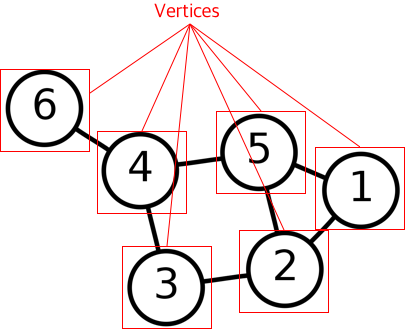
\includegraphics[width=0.4\linewidth]{images/worksheet_4_solution_1.png}
            \end{center}
        \end{itemize}

        \item \textbf{Adjacency-list Representation}
        \begin{itemize}
            \item Associates each vertax in a graph with the collection of its neighbouring vertices or edges
            \item Is represented by $Adj[v]$
            \begin{itemize}
                \item Means all vertices that are neighbour to vertex $v$
                \item In a directed graph, $Adj[v]$ are all out-degree vertices of vertax $v$
                \item $\lvert Adj[v] \rvert$ means the total number of outdegree of vertax $v$
            \end{itemize}
        \end{itemize}

        \begin{center}
        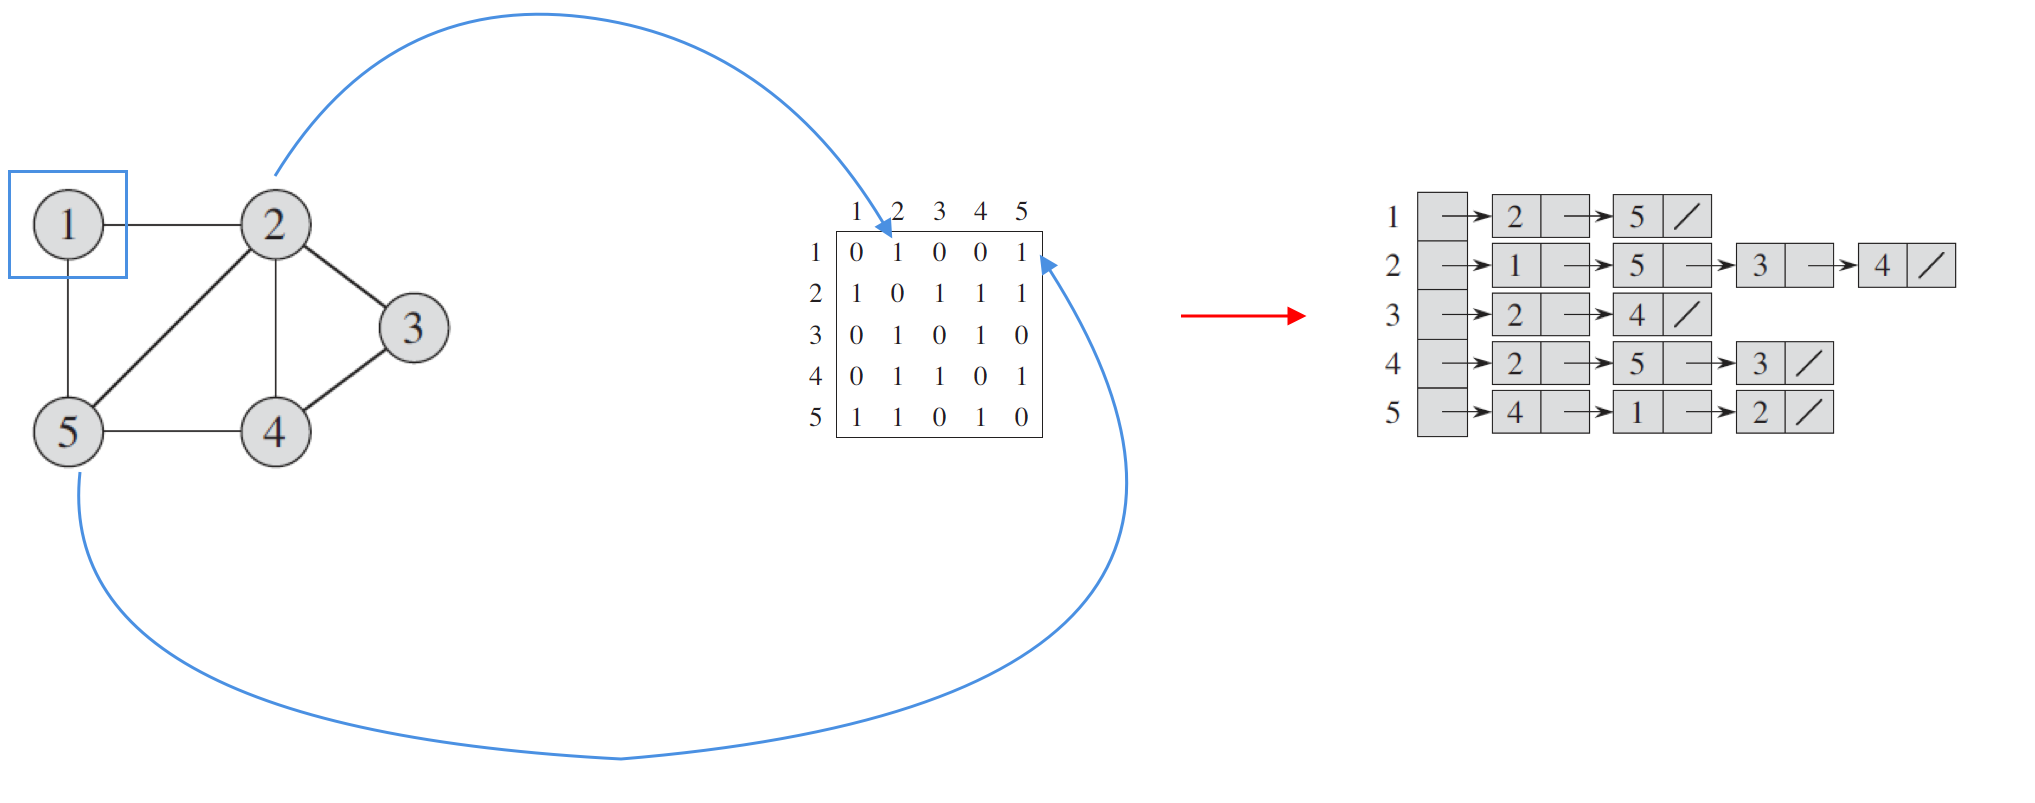
\includegraphics[width=\linewidth]{images/worksheet_4_solution_2.png}
        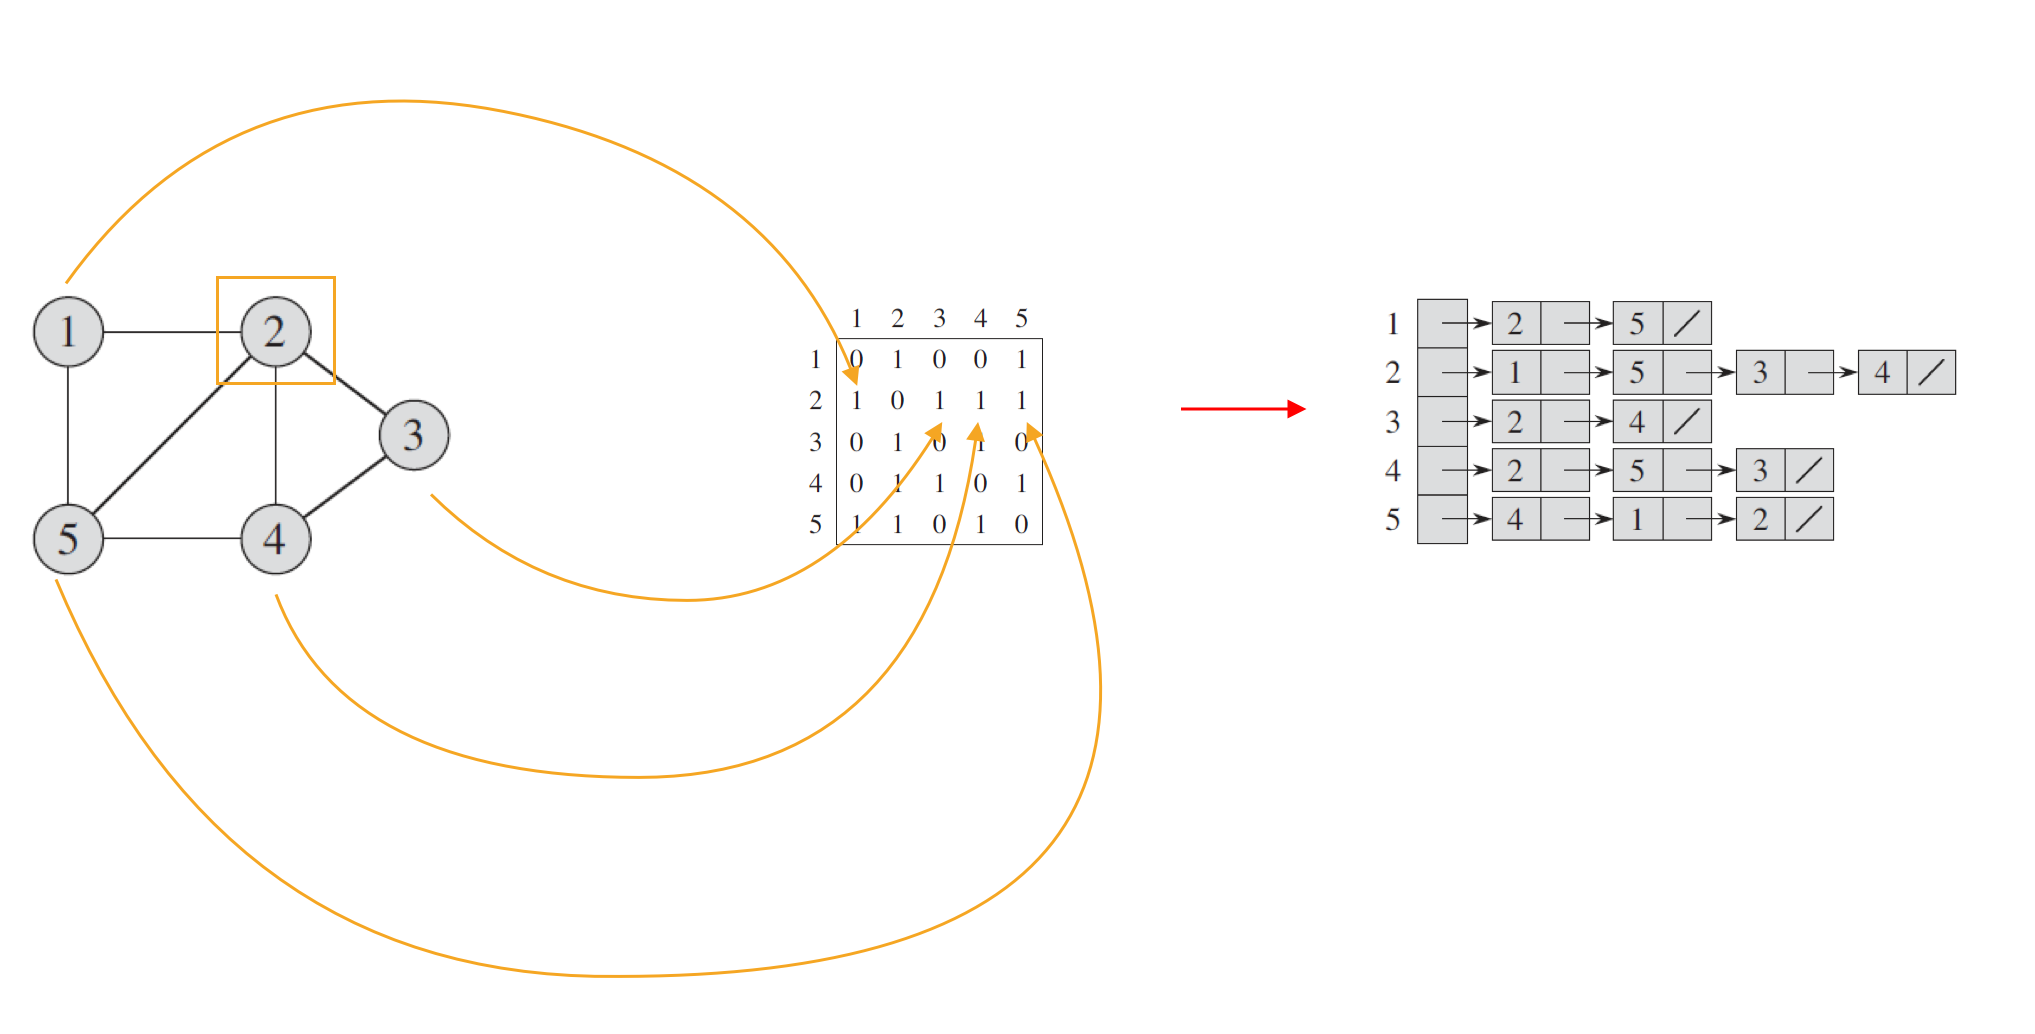
\includegraphics[width=\linewidth]{images/worksheet_4_solution_3.png}
        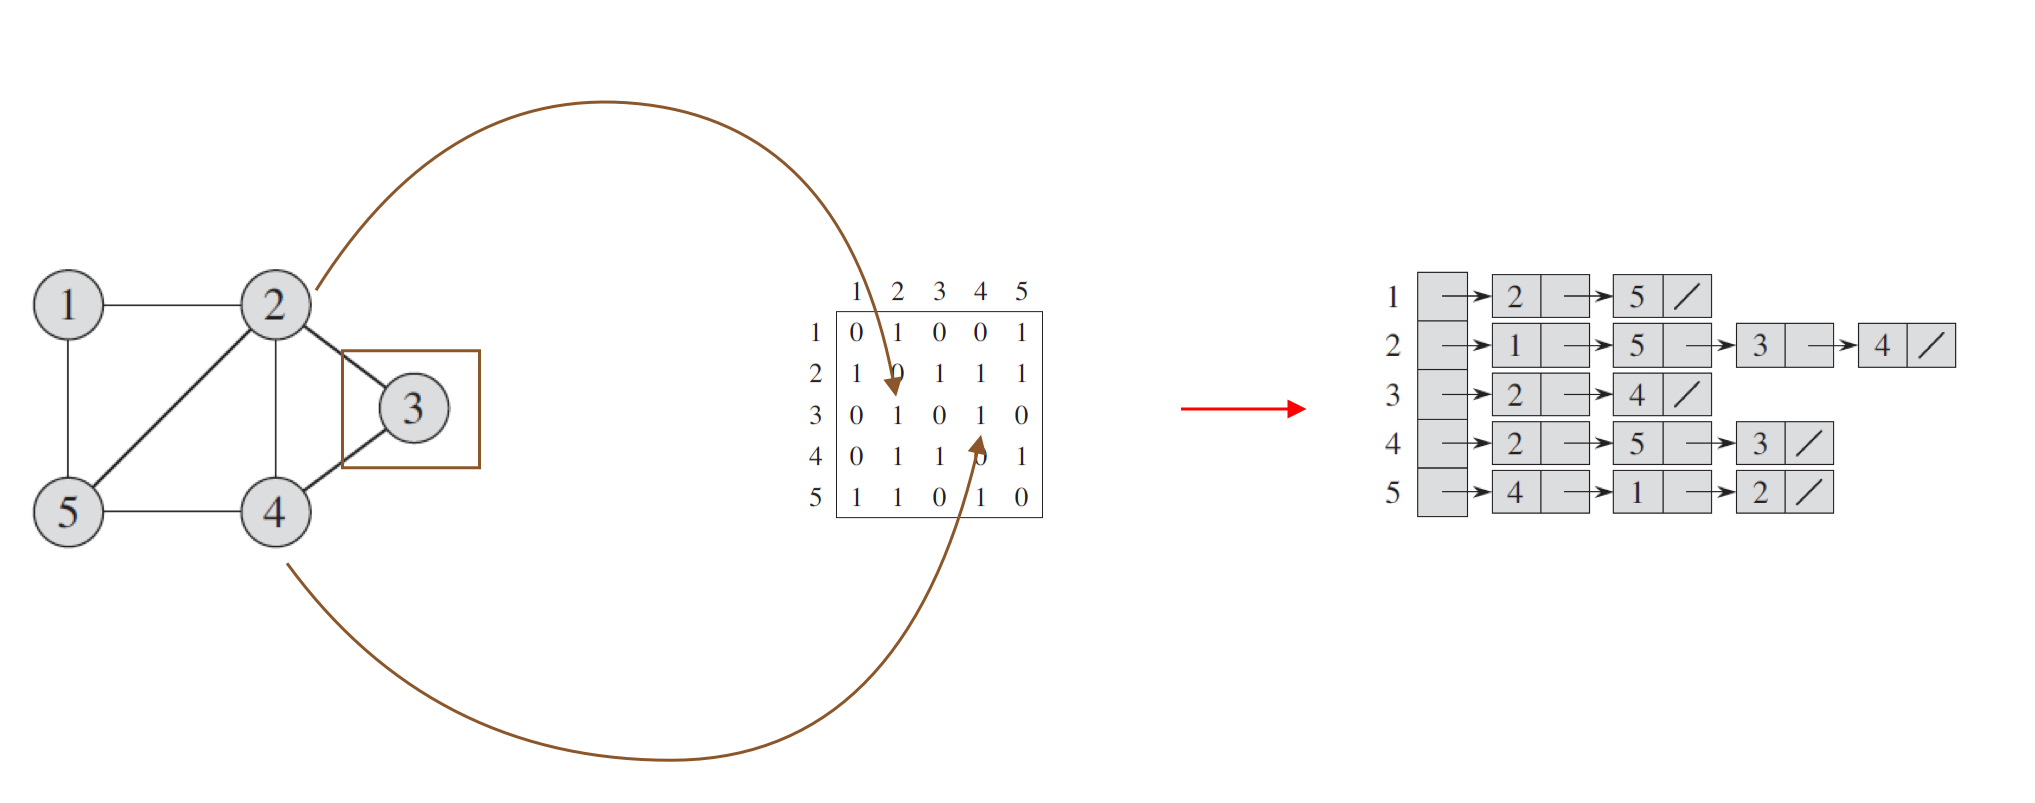
\includegraphics[width=\linewidth]{images/worksheet_4_solution_4.png}
        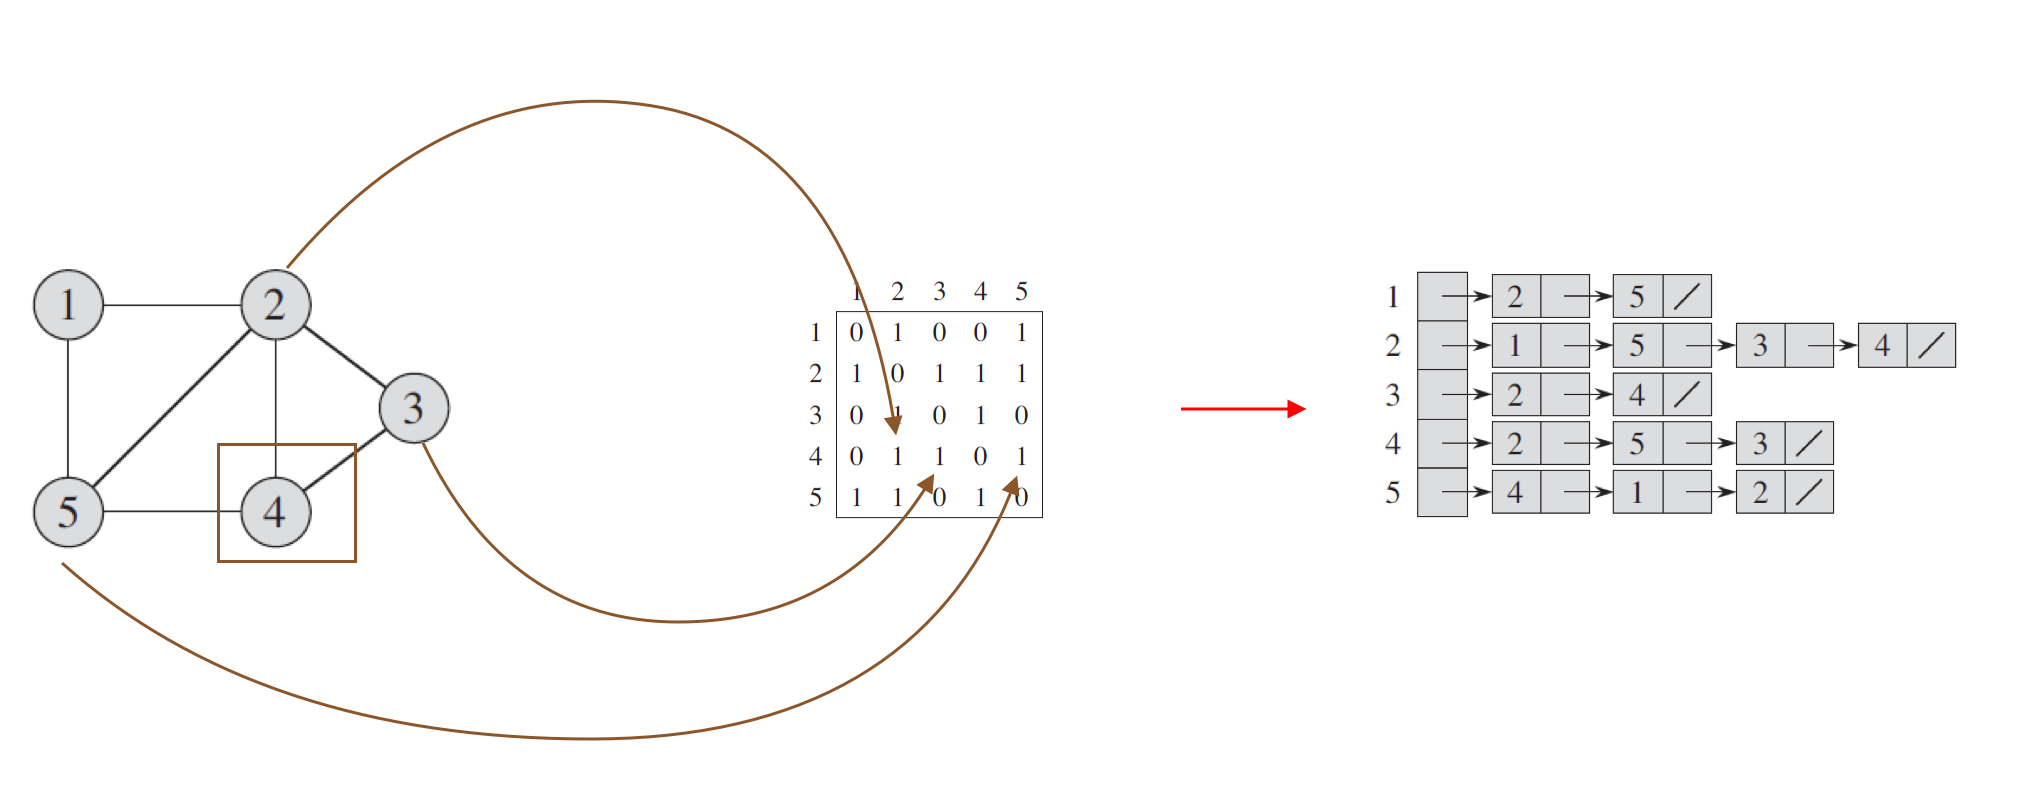
\includegraphics[width=\linewidth]{images/worksheet_4_solution_5.png}
        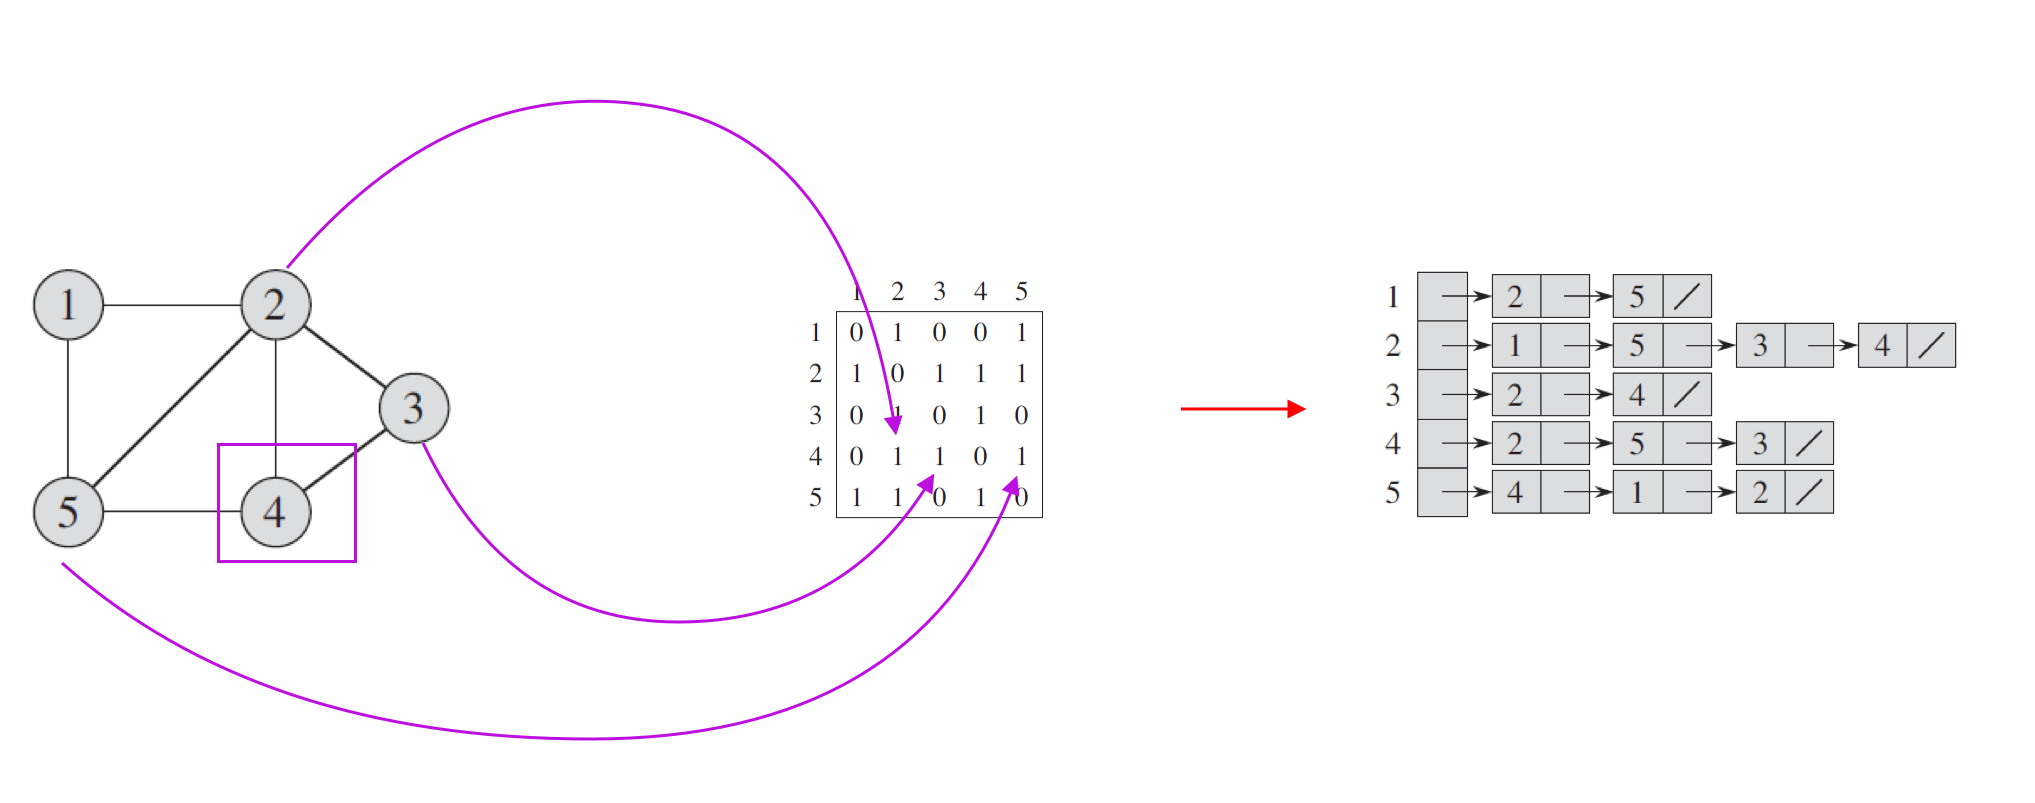
\includegraphics[width=\linewidth]{images/worksheet_4_solution_6.png}
        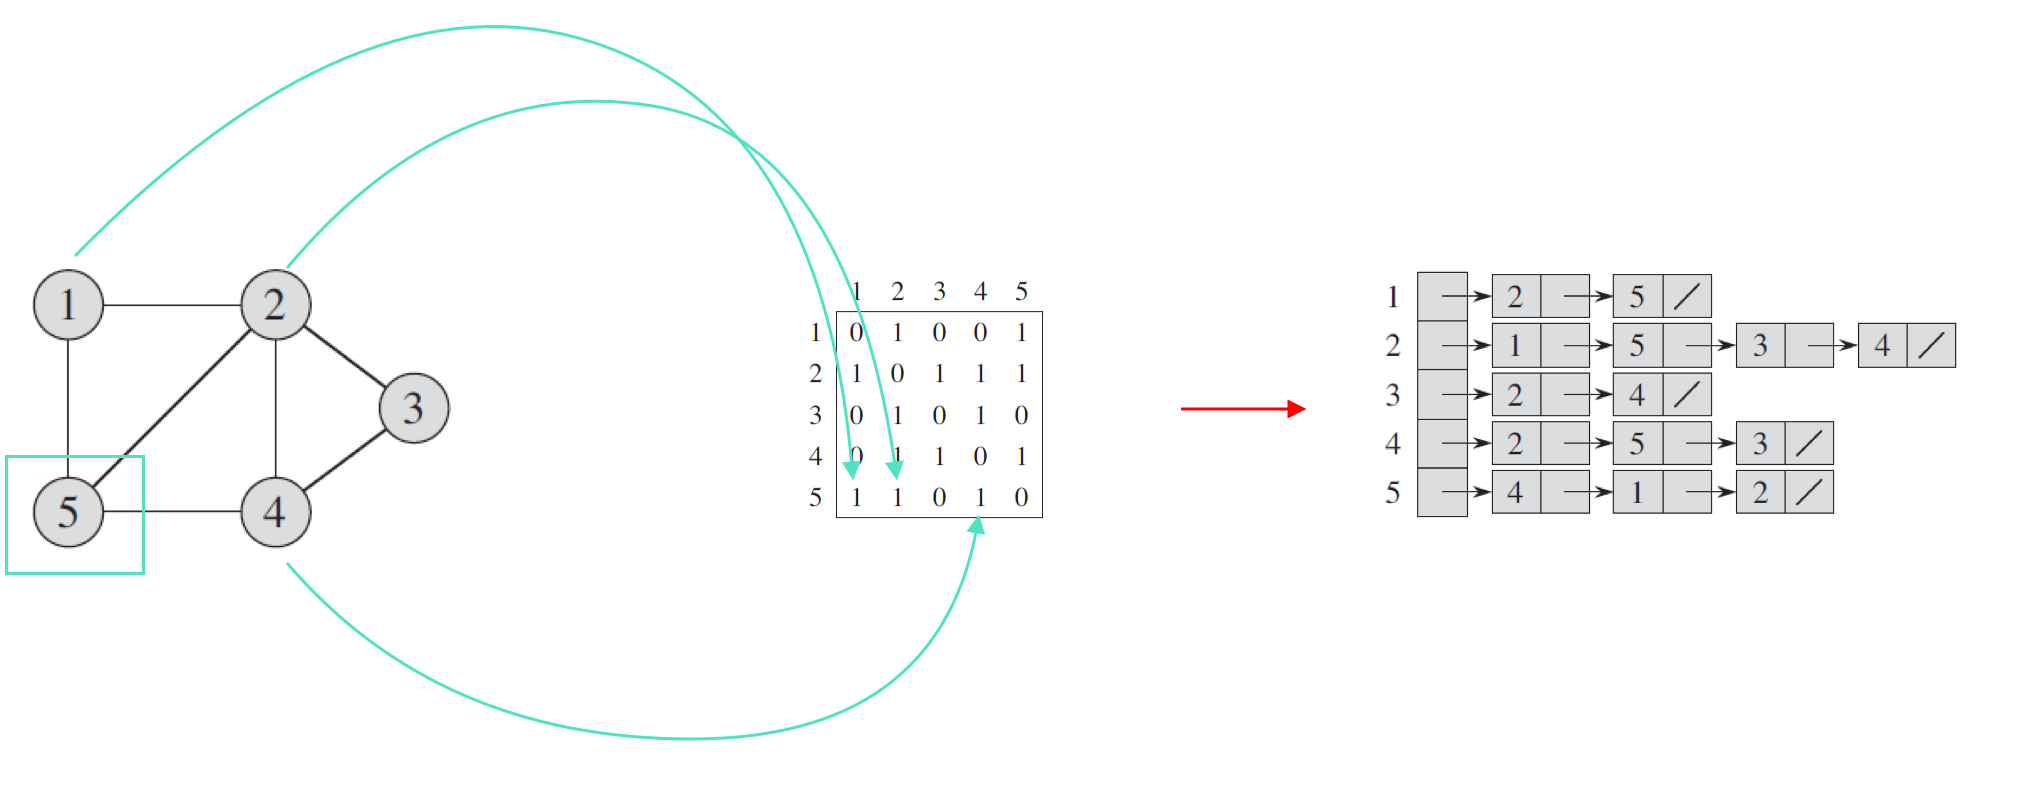
\includegraphics[width=\linewidth]{images/worksheet_4_solution_7.png}
        \end{center}

        \item \textbf{Directed graph}
        \begin{itemize}
            \item Is a graph that is made up of a set of vertices connected by edges,
            where the edges have a direction associated with them

            \begin{center}
            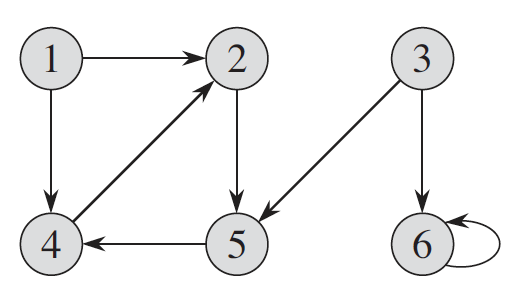
\includegraphics[width=0.4\linewidth]{images/worksheet_4_solution_8.png}
            \end{center}
        \end{itemize}

        \item \textbf{Out-degrees}
        \begin{itemize}
            \item For a directed graph $G=(V(G),E(G))$ and a vertex $x_1 \in V(G)$,
            the Out-Degree of $x_1$ refers to the number of arcs incident from $x_1$.
            That is, the number of arcs directed \underline{away} from the vertex $x_1$.

            \begin{center}
            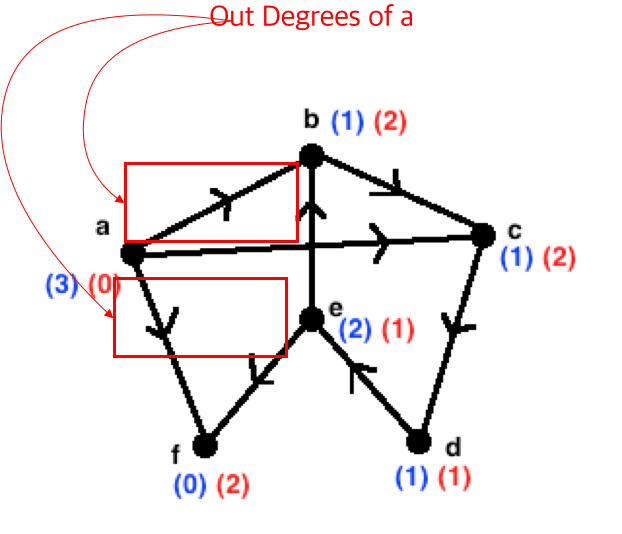
\includegraphics[width=0.4\linewidth]{images/worksheet_4_solution_9.png}
            \end{center}
        \end{itemize}

        \item \textbf{In-degrees}
        \begin{itemize}
            \item For a directed graph $G=(V(G),E(G))$ and a vertex $x_1 \in V(G)$,
            the In-Degree of $x_1$ refers to the number of arcs incident to $x_1$.
            That is, the number of arcs directed \underline{towards} the vertex $x_1$.

            \begin{center}
            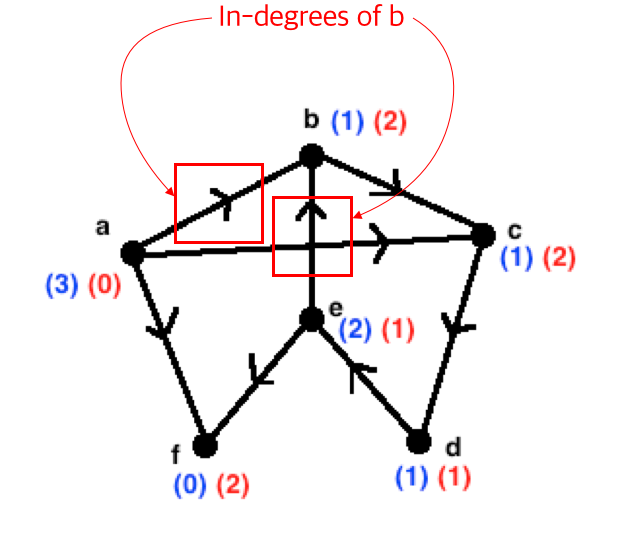
\includegraphics[width=0.4\linewidth]{images/worksheet_4_solution_10.png}
            \end{center}
        \end{itemize}

        \item Computing the outdegree of every vertex using adjacency list

        \bigskip

        \begin{center}
        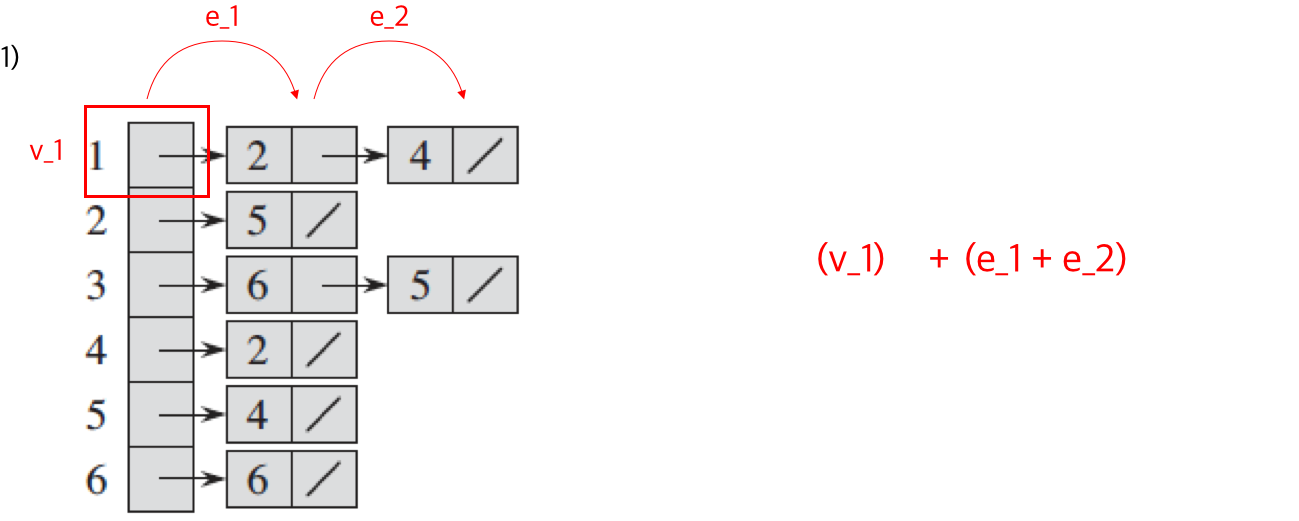
\includegraphics[width=\linewidth]{images/worksheet_4_solution_11.png}
        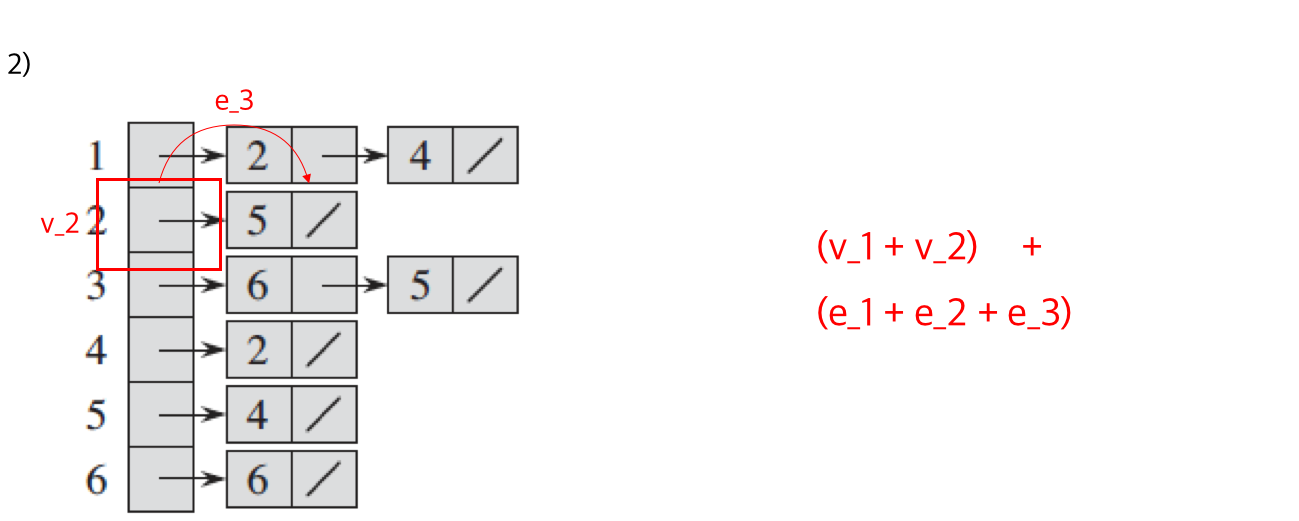
\includegraphics[width=\linewidth]{images/worksheet_4_solution_12.png}
        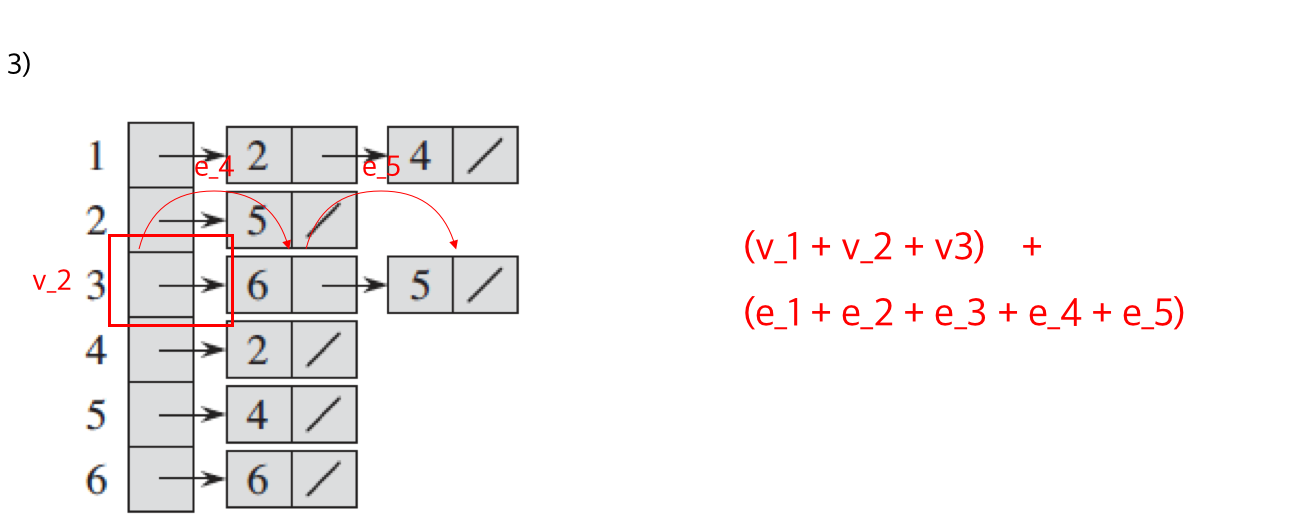
\includegraphics[width=\linewidth]{images/worksheet_4_solution_13.png}
        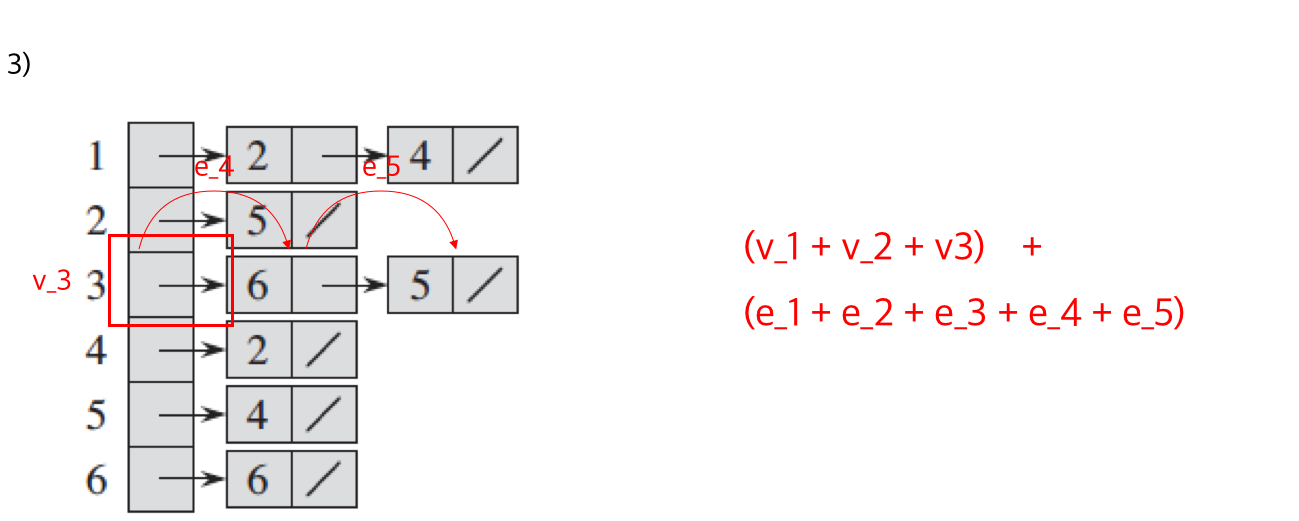
\includegraphics[width=\linewidth]{images/worksheet_4_solution_14.png}
        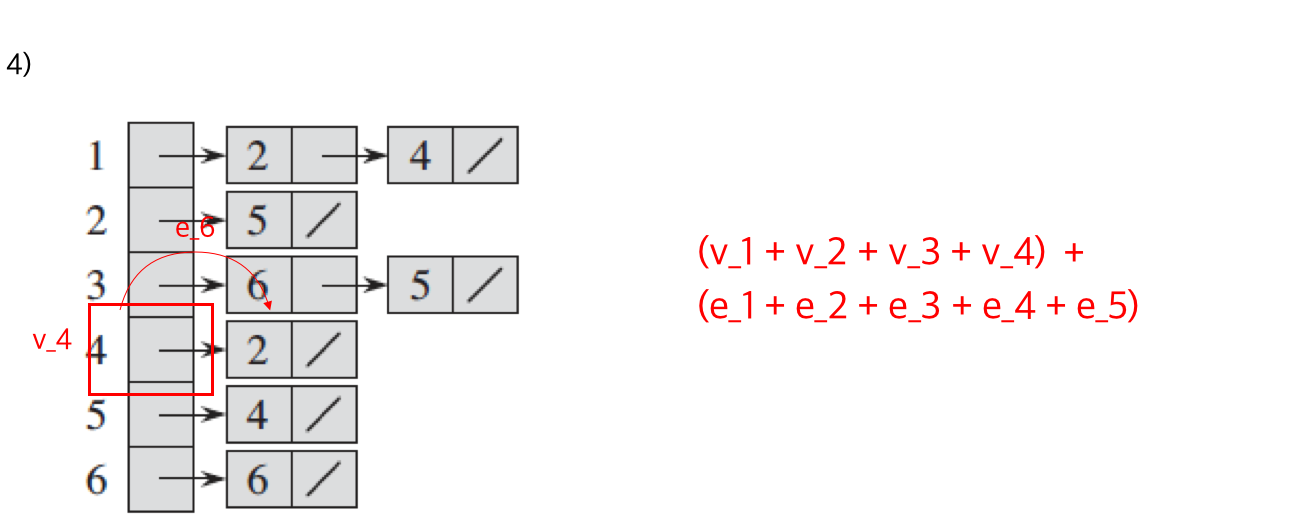
\includegraphics[width=\linewidth]{images/worksheet_4_solution_15.png}
        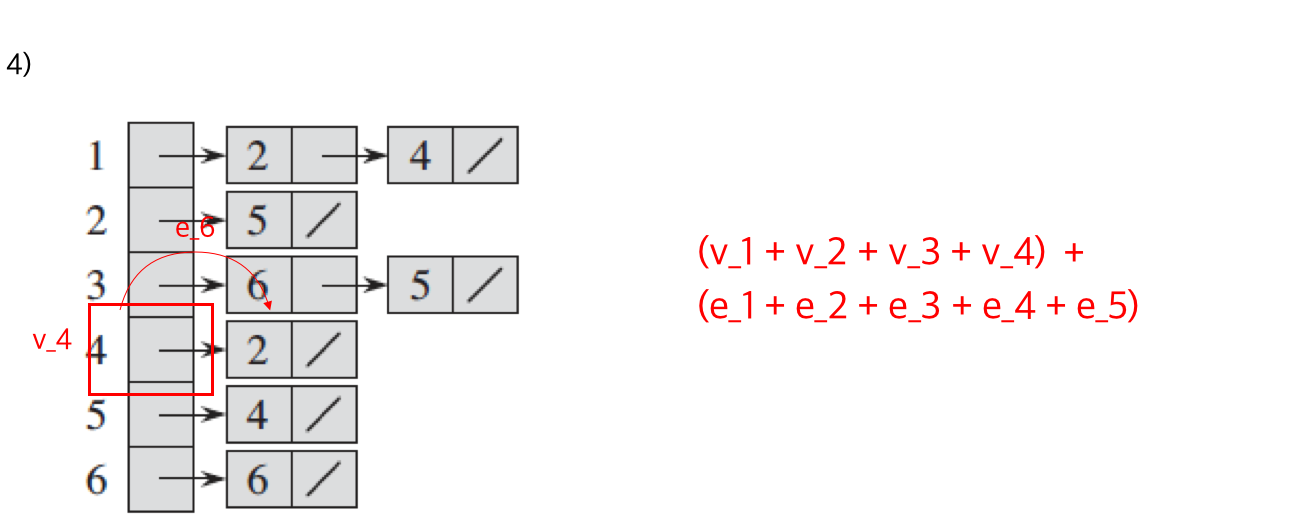
\includegraphics[width=\linewidth]{images/worksheet_4_solution_16.png}
        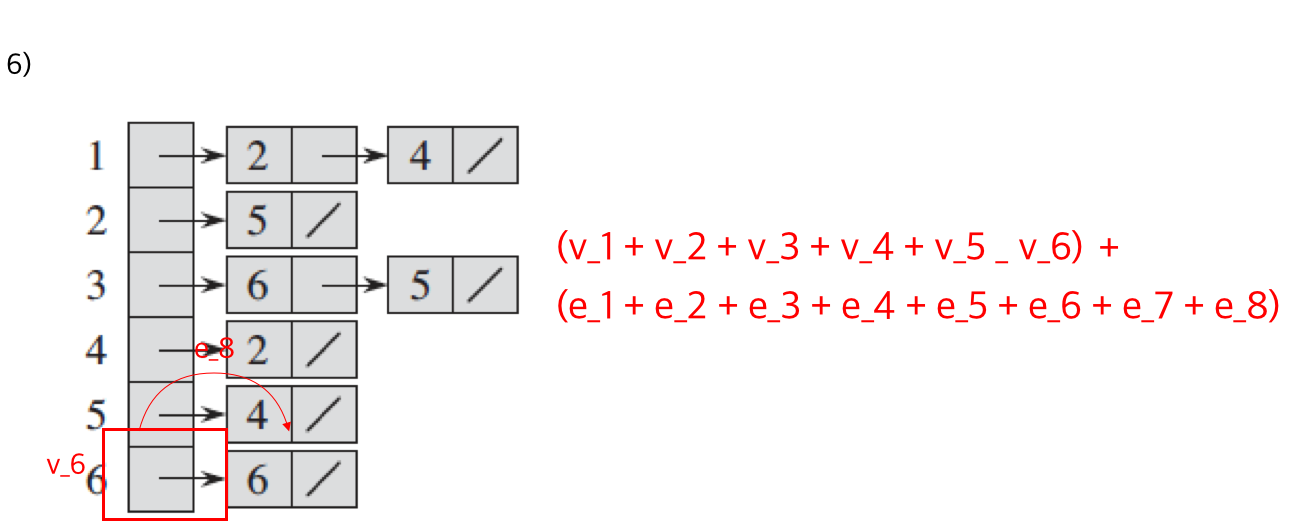
\includegraphics[width=\linewidth]{images/worksheet_4_solution_17.png}
        \end{center}

        \bigskip

        So it has $\mathcal{O}(V + E)$

        \item Computing the outdegree of every vertex using adjacency list

        \bigskip

        The outdegree of a vertex is indegree of another vertex.

        \bigskip

        Using this fact, we can conclude the running time of computing indegree of every vertax is $\mathcal{O}(V + E)$.
    \end{itemize}

    \item

    \begin{itemize}
        \item Computing $G^T$ from $G$ in Adjacency List

        \begin{center}
        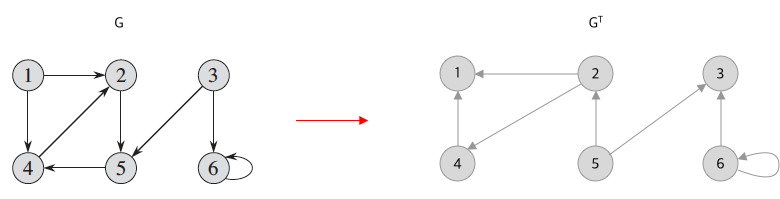
\includegraphics[width=\linewidth]{images/worksheet_4_solution_18.png}
        \end{center}

    \begin{lstlisting}[mathescape=true]
    COMPUTE-G-TRANSPOSE-ADJ-MATRIX(Adj,V)
        Let Adj' be a new adjacency list containing keys $v_i...v_n$

        for i = 1 to $\lvert V \rvert$
            for every vertax $w$ in Adj[$v_i$]
                Insert(Adj'[w], $v_i$)

        return Adj'
    \end{lstlisting}

        \item Computing $G^T$ from $G$ in Adjacency-Matrix

        \begin{center}
        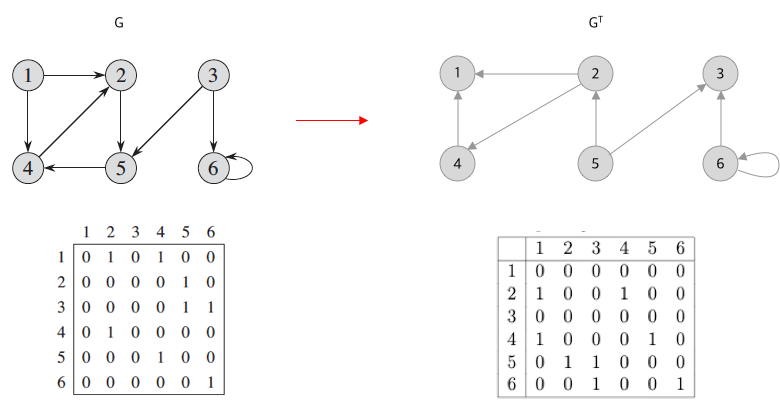
\includegraphics[width=\linewidth]{images/worksheet_4_solution_19.png}
        \end{center}

    \begin{lstlisting}[mathescape=true]
    COMPUTE-G-TRANSPOSE-ADJ-MATRIX(A,V)
        Let A'[1..$\lvert V \rvert$, 1..$\lvert V \rvert$] be a new adjacency matrix

        for i = 1 to $\lvert V \rvert$
            for j = 1 to $\lvert V \rvert$
                A'[j,i] = A[i,j]

        return A'
    \end{lstlisting}

    \bigskip

    \end{itemize}

    \bigskip


    \begin{mdframed}
        \underline{\textbf{Correct Solution:}}

        \bigskip

        \begin{itemize}
            \item Computing $G^T$ from $G$ in Adjacency List

            \begin{center}
            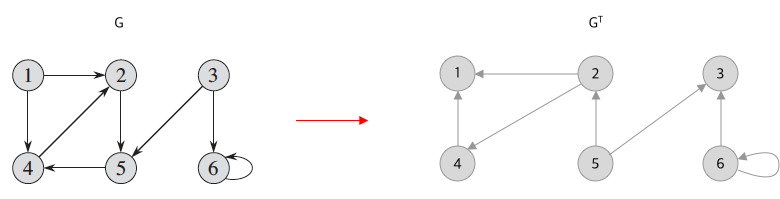
\includegraphics[width=\linewidth]{images/worksheet_4_solution_18.png}
            \end{center}

        \begin{lstlisting}[mathescape=true]
        COMPUTE-G-TRANSPOSE-ADJ-MATRIX(Adj,V)
            Let Adj' be a new adjacency list containing keys $v_i...v_n$

            for i = 1 to $\lvert V \rvert$
                for every vertax $w$ in Adj[$v_i$]
                    Insert(Adj'[w], $v_i$)

            return Adj'
        \end{lstlisting}

            \bigskip

            \color{red}The running time is $\mathcal{O}(\lvert V \rvert + \lvert E \rvert)$\color{black}

            \item Computing $G^T$ from $G$ in Adjacency-Matrix

            \begin{center}
            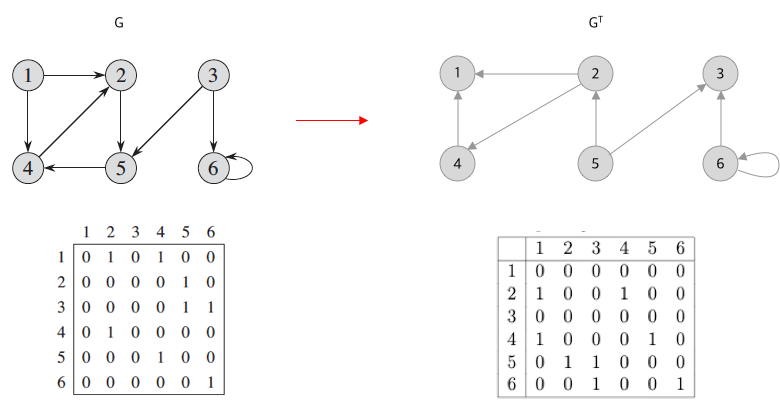
\includegraphics[width=\linewidth]{images/worksheet_4_solution_19.png}
            \end{center}

        \begin{lstlisting}[mathescape=true]
        COMPUTE-G-TRANSPOSE-ADJ-MATRIX(A,V)
            Let A'[1..$\lvert V \rvert$, 1..$\lvert V \rvert$] be a new adjacency matrix

            for i = 1 to $\lvert V \rvert$
                for j = 1 to $\lvert V \rvert$
                    A'[j,i] = A[i,j]

            return A'
        \end{lstlisting}

        \bigskip

        \color{red}The running time is $\mathcal{O}(\lvert V \rvert^2)$\color{black}


        \end{itemize}
    \end{mdframed}


    \item

    \bigskip

    \begin{lstlisting}[mathescape=true]
    Breadth-First-Search(V,$v_i$)
        d = 0
        for each $v_i \in V$
            while performing BFS(V, $v_i$)
                let $w$ be the current node in BFS
                    if $\delta($v_i$,w) > d$
                        d = $\delta(v_i, w)$

        return d
    \end{lstlisting}

    \bigskip

    \underline{Finding Runtime of Algorithm}

    \bigskip

    Since the graph iterates $\sum\limits_{i=1}^n Adj[v_i] = \lvert E \rvert$
    times for each $v_i \in V$, the algorithm iterates total of $\lvert V \rvert \cdot \lvert E \rvert$ times,
    which is $\mathcal{O}(\lvert V \rvert \lvert E \rvert)$.


    \bigskip

    \underline{\textbf{Notes:}}

    \bigskip

    \begin{itemize}
        \item \textbf{Breadth First Search}

        \begin{itemize}
            \item Is an algorithm for searching or traversing a graph
            \item Is one of the simplest algorithm
        \end{itemize}

        \item \textbf{Largest of All Shortest Path Distance}

        \bigskip

        \begin{itemize}
            \item Means the shortest distance between two furthest apart nodes

            \bigskip

            \begin{center}
            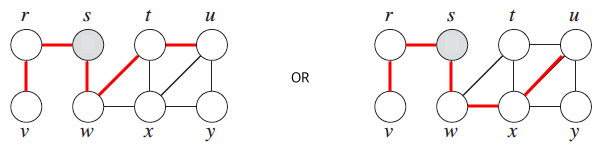
\includegraphics[width=\linewidth]{images/worksheet_4_solution_20.png}
            \end{center}
        \end{itemize}
    \end{itemize}

    \bigskip

    \underline{\textbf{References}}

    \bigskip

    \begin{enumerate}[1)]
        \item McGill University, 308-360 Tutorial, \href{https://www.cs.mcgill.ca/~kaleigh/teaching/360_tutorials/tutorial_02.html}{link}
    \end{enumerate}

    \item

    \bigskip

    \begin{center}
    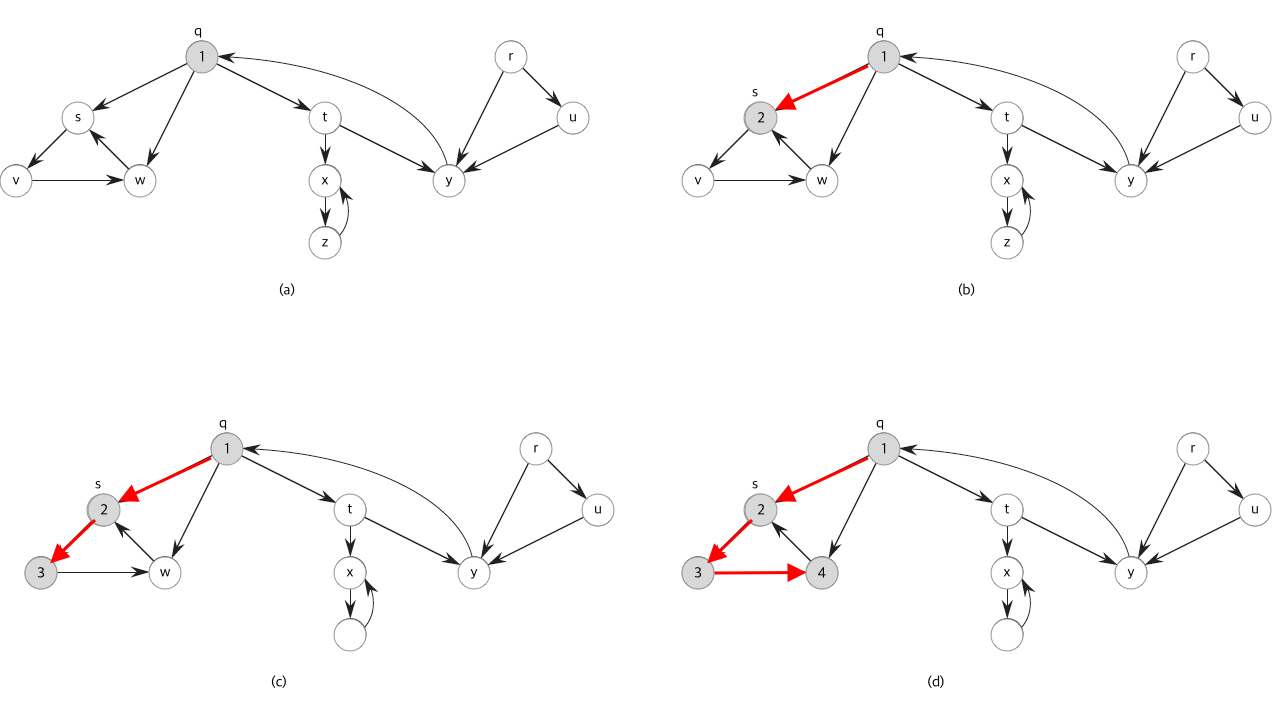
\includegraphics[width=\linewidth]{images/worksheet_4_solution_21.png}
    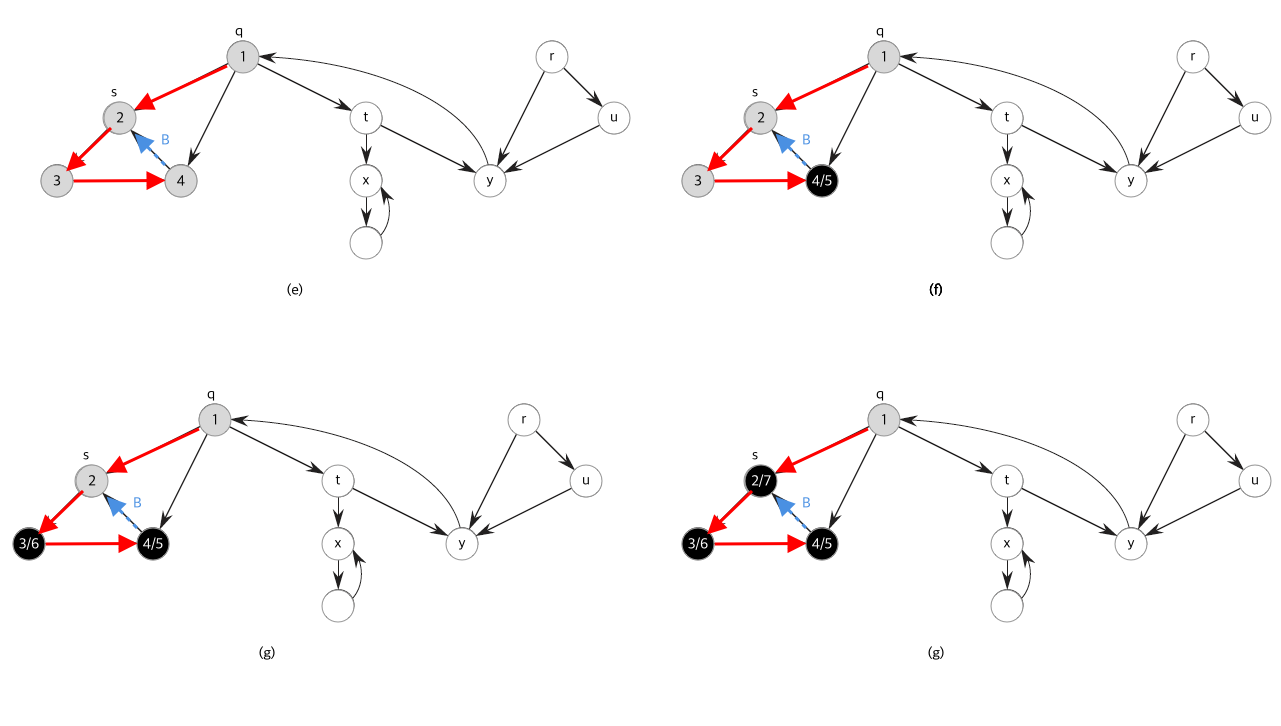
\includegraphics[width=\linewidth]{images/worksheet_4_solution_22.png}
    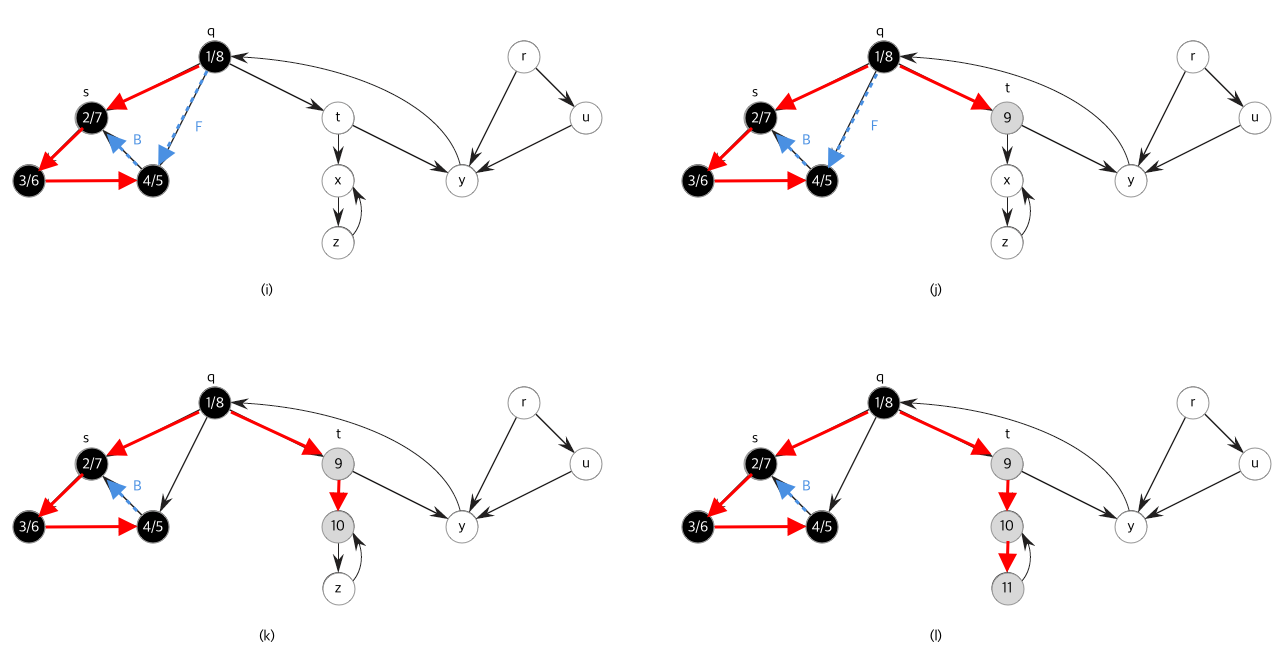
\includegraphics[width=\linewidth]{images/worksheet_4_solution_26.png}
    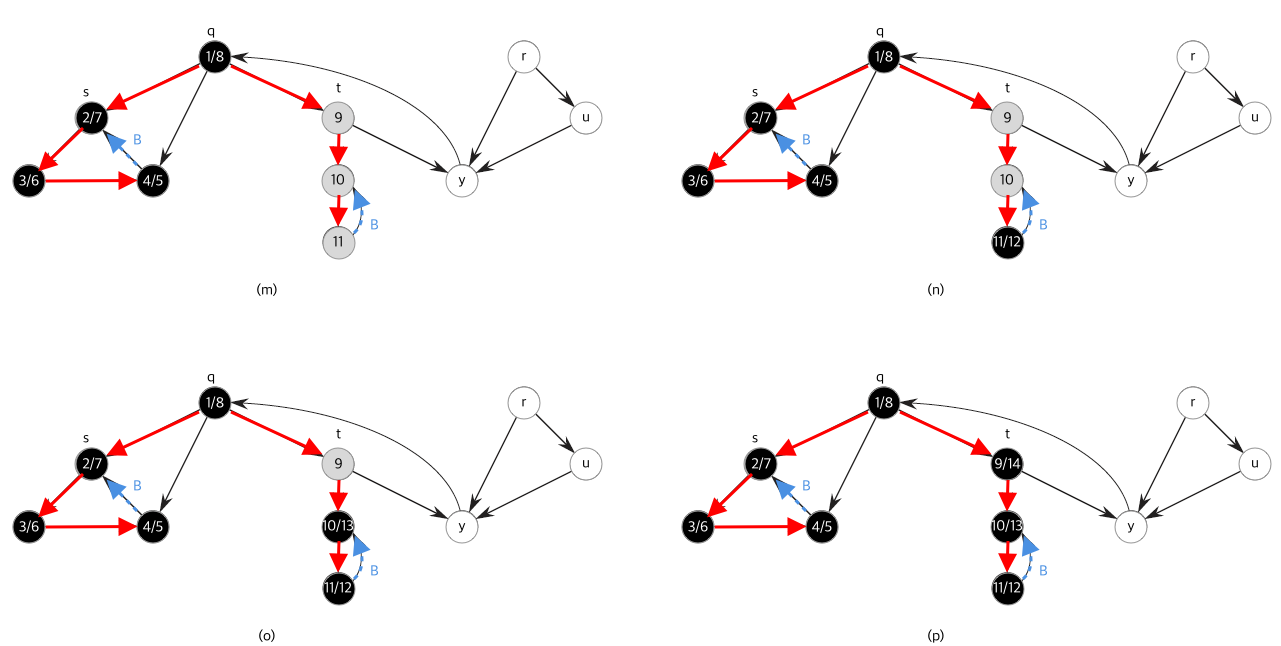
\includegraphics[width=\linewidth]{images/worksheet_4_solution_27.png}
    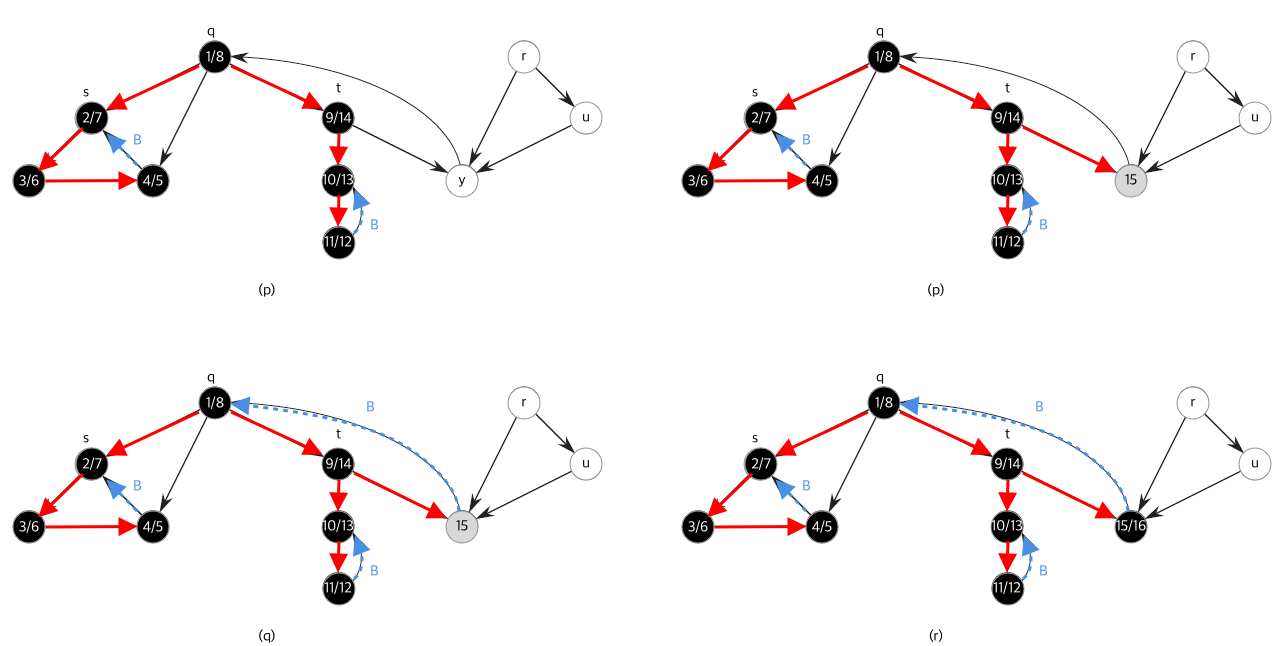
\includegraphics[width=\linewidth]{images/worksheet_4_solution_28.png}
    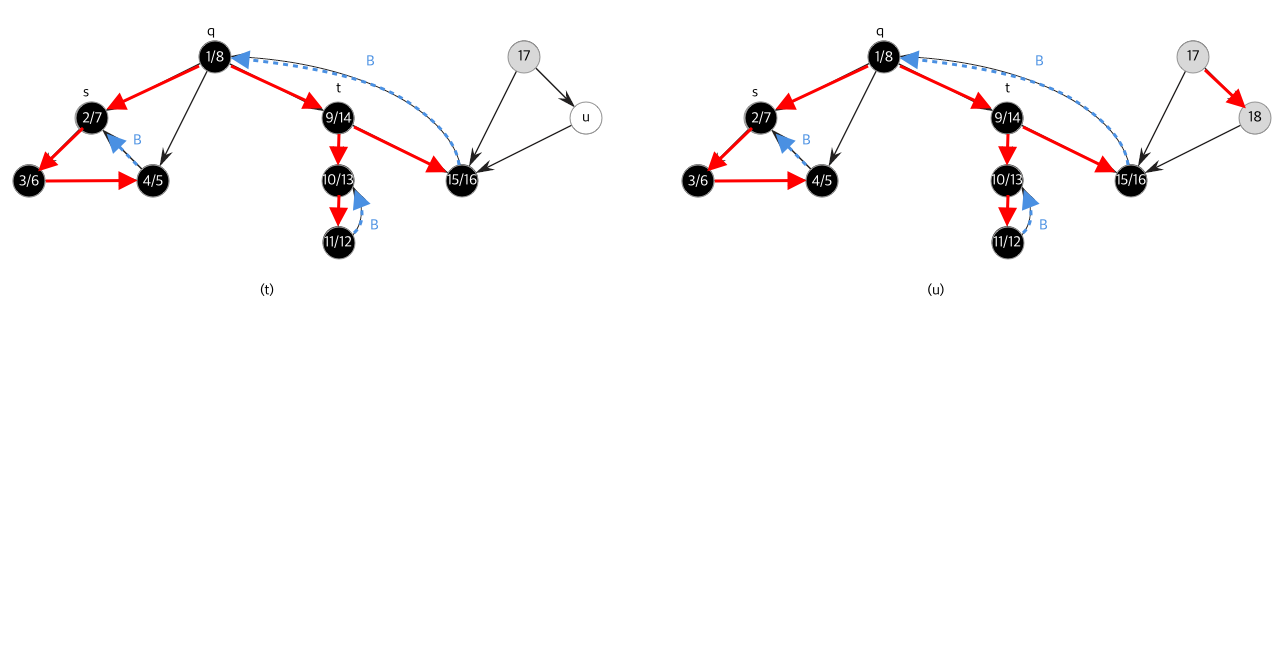
\includegraphics[width=\linewidth]{images/worksheet_4_solution_29.png}
    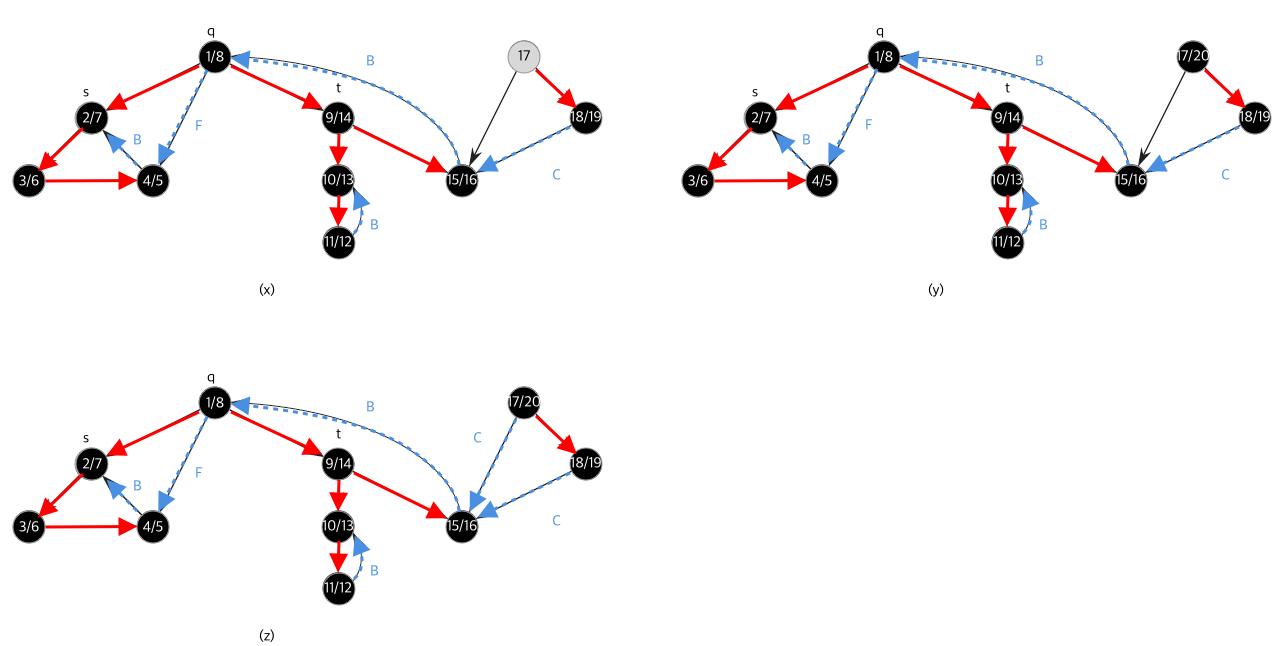
\includegraphics[width=\linewidth]{images/worksheet_4_solution_30.png}
    \end{center}

    \bigskip

    \underline{\textbf{Notes:}}

    \bigskip

    \begin{itemize}
        \item \textbf{Depth First Search}

        \begin{itemize}
            \item Searches deeper in the graph whenever possible
        \end{itemize}

        \item \textbf{Forward Edge}

        \begin{itemize}
            \item Is an edge $(u,v)$ such that $v$ is descendant but not part of
            the DFS tree. Edge $1 \to 8$ is a foward edge

            \begin{center}
            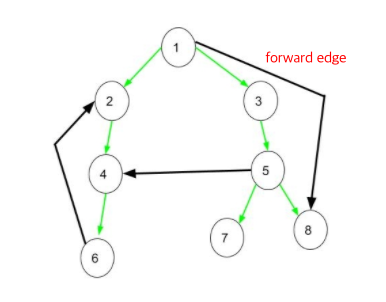
\includegraphics[width=0.6\linewidth]{images/worksheet_4_solution_23.png}
            \end{center}
         \end{itemize}

         \item \textbf{Back Edge}

        \begin{itemize}
            \item It is an edge $(u, v)$ such that $v$ is ancestor of edge $u$
            but not part of DFS tree. Edge from $6 \to 2$ is a back edge.
            \item Indicates a cycle in a graph

            \begin{center}
            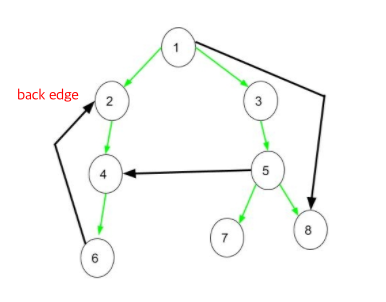
\includegraphics[width=0.6\linewidth]{images/worksheet_4_solution_24.png}
            \end{center}

        \end{itemize}

        \item \textbf{Cross Edge}

        \begin{itemize}
            \item It is a edge which connects two node such that they do not
            have any ancestor and a descendant relationship between them.
            Edge from node $5 \to 4$ is cross edge.

            \begin{center}
            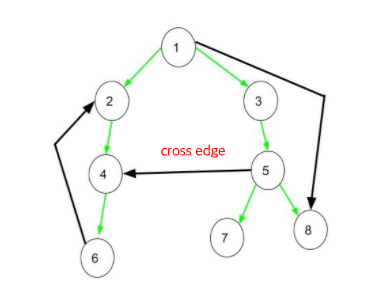
\includegraphics[width=0.6\linewidth]{images/worksheet_4_solution_25.png}
            \end{center}
        \end{itemize}
    \end{itemize}

    \underline{\textbf{References}}

    \bigskip

    \begin{enumerate}[1)]
        \item Geeks For Geeks, Tree, Back, Edge and Cross Edges in DFS of Graph, \href{https://www.geeksforgeeks.org/tree-back-edge-and-cross-edges-in-dfs-of-graph/}{link}
    \end{enumerate}

    \item

    \bigskip

    \begin{proof}
    Let $G$ be a connectded graph. Let $A$ be a subset of $E$ that is always included
    in some minimum spanning treee for $G$.

    \bigskip

    Assume for the sake of contradiction that $(u,v)$ is not contained in some
    minimum spanning tree of $G$.

    \bigskip

    We know from the minimum-spanning tree algorithm that a light edge crossings in a
    cut of $G$ that respects $A$ is always chosen (since this is a safe edge and the
    algorithm always picks the safe edge).

    \bigskip

    Since the edge $(u,v)$ is not a part of minimum spanning tree, $(u,v)$
    is not chosen in a cut.

    \bigskip

    Since $(u,v)$ is not chosen, the edge $(u',v')$ with smaller weight
    is chosen.

    \bigskip

    Then this violates the assumption that $(u,v)$ is the edge with the smallest weight.

    \bigskip

    Thus, by contradiction, $(u,v)$ belongs to some minimum spanning tree of $G$.

    \end{proof}

    % \bigskip

    % \underline{\textbf{Rough Work}}

    % \bigskip

    % Let $G$ be a connectded graph. Let $A$ be a subset of $E$ that is always included
    % in some minimum spanning treee for $G$.

    % \bigskip

    % Assume for the sake of contradiction that $(u,v)$ is not contained in some
    % minimum spanning tree of $G$.

    % \bigskip

    % \begin{enumerate}[1.]
    %     \item State that the minimum spanning algorithm always picks the edge with
    %     smallest weight in a cut between growing minimum spanning Tree $(V - S)$ and
    %     the set of vertices $S$

    %     \begin{mdframed}
    %     We know from the minimum-spanning tree algorithm that a light edge crossings in a
    %     cut of $G$ that respects $A$ is always chosen (since this is a safe edge and the
    %     algorithm always picks the safe edge).

    %     \end{mdframed}

    %     \item State that since $(u,v)$ is not a part of minimum spanning tree, $(u,v)$
    %     is not chosen in a cut.

    %     \begin{mdframed}
    %     Since the edge $(u,v)$ is not a part of minimum spanning tree, $(u,v)$
    %     is not chosen in a cut.
    %     \end{mdframed}

    %     \item State that since $(u,v)$ is not chosen, the edge $(u',v')$ with smaller weight
    %     is chosen

    %     \begin{mdframed}
    %     Since $(u,v)$ is not chosen, the edge $(u',v')$ with smaller weight
    %     is chosen
    %     \end{mdframed}

    %     \item This violates the assumption that $(u,v)$ is the edge with the smallest weight.

    %     \begin{mdframed}
    %     Then this violates the assumption that $(u,v)$ is the edge with the smallest weight.
    %     \end{mdframed}

    %     \item Thus, by contradiction, $(u,v)$ belongs to some minimum spanning tree of $G$.

    %     \begin{mdframed}
    %     Thus, by contradiction, $(u,v)$ belongs to some minimum spanning tree of $G$.
    %     \end{mdframed}
    % \end{enumerate}

    \bigskip

    \underline{\textbf{Notes:}}

    \bigskip

    \begin{itemize}
        \item \textbf{Spanning Tree}

        \bigskip

        Given an undirected and connected graph $G = (V,E)$, a spanning tree of
        the graph $G$ is a tree that spans $G$ (that is, it includes every vertex
        of $G$) and is a subgraph of $G$ (every edge in the tree belongs to $G$)

        \bigskip

        \begin{center}
        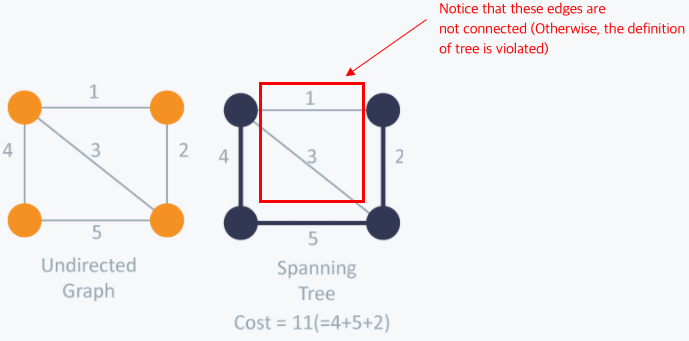
\includegraphics[width=0.7\linewidth]{images/worksheet_4_solution_31.png}
        \end{center}
        \item \textbf{Minimum Spanning Tree}

        \begin{itemize}
            \item Is the spanning tree where the \underline{cost is minimum} among all the spanning trees.
            \begin{itemize}
                \item The cost of the spanning tree is the sum of the weights of all the edges in the tree.
            \end{itemize}
            \item There can be many minimum spanning trees.

            \begin{center}
            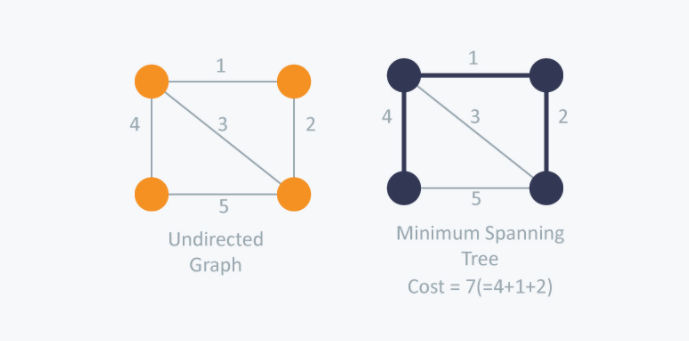
\includegraphics[width=0.7\linewidth]{images/worksheet_4_solution_32.png}
            \end{center}
            \item Is used in
            \begin{enumerate}[1.]
                \item Network design (Telephone, electrical, hydraulic, TV cable, computer, road)
                \item Approximation algorithm for NP-hard problems
                \item Learning sailent features for real-time face verification
                \item Reducing data storage in sequencing amino acids in a protein
            \end{enumerate}
        \end{itemize}

        \begin{center}
        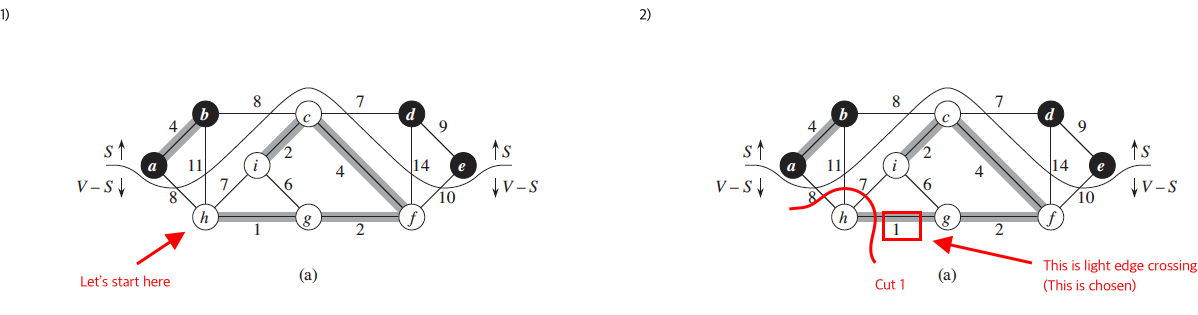
\includegraphics[width=\linewidth]{images/worksheet_4_solution_35.png}
        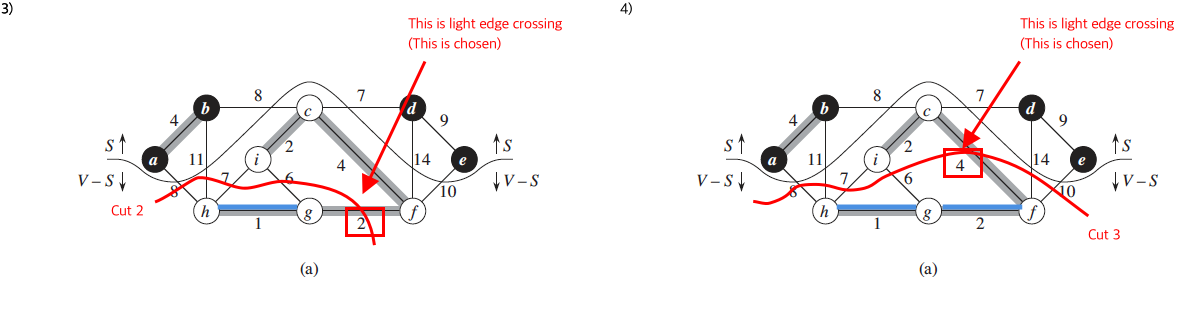
\includegraphics[width=\linewidth]{images/worksheet_4_solution_36.png}
        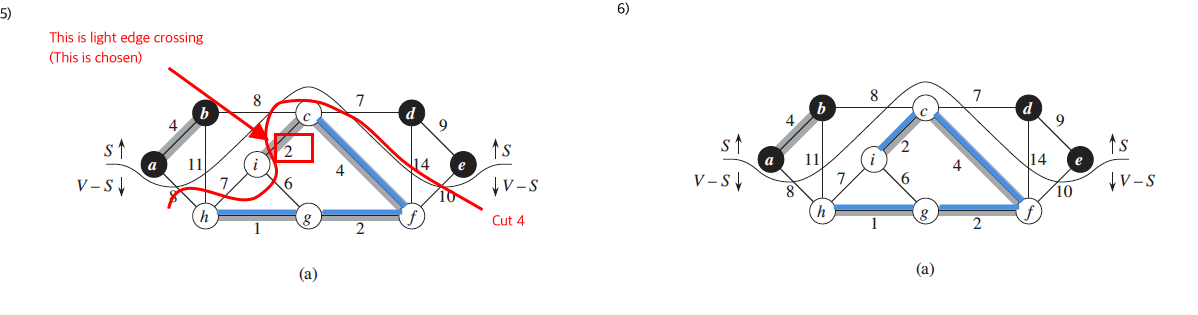
\includegraphics[width=\linewidth]{images/worksheet_4_solution_37.png}
        \end{center}

        \item \textbf{Cut}

        \begin{itemize}
            \item A cut of an undirected graph $G = (V,E)$ is denoted $(S, V - S)$
            \item Is a partition of $V$

            \begin{center}
            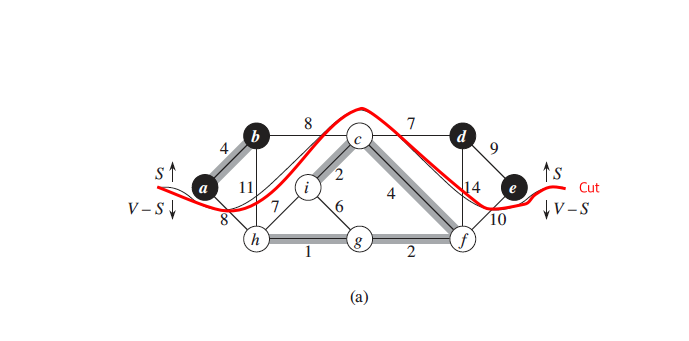
\includegraphics[width=0.8\linewidth]{images/worksheet_4_solution_33.png}
            \end{center}
        \end{itemize}

        \item \textbf{Light Edge Crossing}
        \begin{itemize}
            \item An edge is a light edge crossing if its weight is the minimum of any
            edge crossing the cut

            \begin{center}
            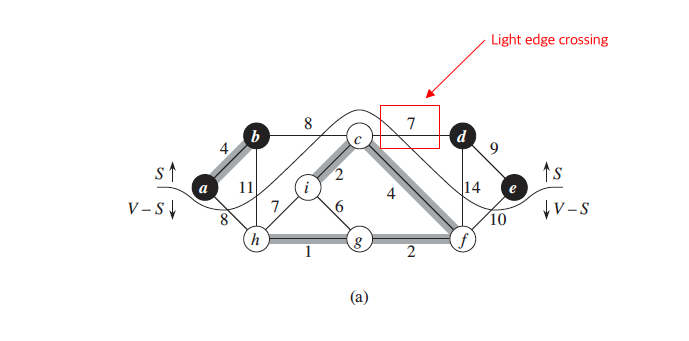
\includegraphics[width=0.8\linewidth]{images/worksheet_4_solution_34.png}
            \end{center}
        \end{itemize}

        \item \textbf{Safe Edge}
        \begin{itemize}
            \item Is an edge $(u,v)$ that may be added to $A$ without violating the invariant that
            $A \cup (u,v)$ is a subset of some minimum spanning tree.
        \end{itemize}

        \item \textbf{Cut respects a set A of edges}

        \begin{itemize}
            \item Means no edges in $A$ crosses the crossing cut

            \begin{center}
            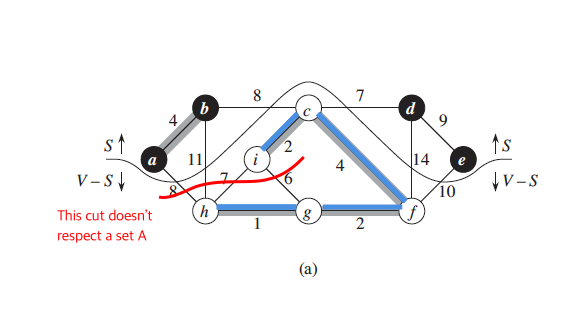
\includegraphics[width=0.8\linewidth]{images/worksheet_4_solution_38.png}
            \end{center}
        \end{itemize}
    \end{itemize}

    \bigskip

    \underline{\textbf{References:}}

    \bigskip

    \begin{enumerate}[1)]
        \item Princeton University, Minimum Spanning Tree, \href{https://www.cs.princeton.edu/courses/archive/spr07/cos226/lectures/mst.pdf}{link}
        \item McGill University, 308-360 Tutorial, \href{https://www.cs.mcgill.ca/~kaleigh/teaching/360_tutorials/tutorial_04.html}{link}
        \item Hacker Earth, Minimum Spanning Tree, \href{https://www.hackerearth.com/practice/algorithms/graphs/minimum-spanning-tree/tutorial/}{link}
    \end{enumerate}


    \item

    \bigskip

    \begin{lstlisting}[mathescape=true]
    MST-PRIM-ADJACENCY-LIST(Adj,w,r)
        Let Q be an empty list
        Q = Extract node objects from Adj

        for i = 1 to $\lvert Q \rvert$
            u.key =  $\infty$
            u.$\pi$ =  NIL

        r.key = 0

        while Q $\neq$ 0
            u = EXTRACT-MIN(Q)
            for each $v \in G.Adj[u]$
                if $v \in Q$ and $w(u,v) < v.key$
                    v.$\pi$ = u
                    v.key = $w(u,v)$
    \end{lstlisting}


    \bigskip

    \underline{\textbf{Notes:}}

    \bigskip

    \begin{itemize}
        \item Kruskal Algorithm

        \begin{itemize}
            \item is a minimum-spanning-tree algorithm which finds an edge of the least possible weight that connects
            any two trees in the forest.
        \end{itemize}

        \item Prim's Algorithm

        \begin{itemize}
            \item Is a greedy algorithm that finds a minimum spanning tree for a
            weighted undirected graph
            \item Is very similar to Dijkstra's algorithm for finding shortest path
            \begin{center}
            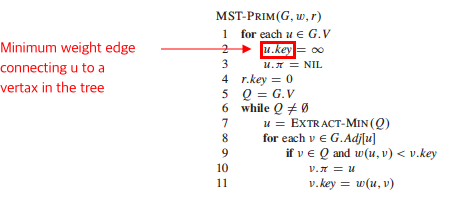
\includegraphics[width=\linewidth]{images/worksheet_4_solution_41.png}
            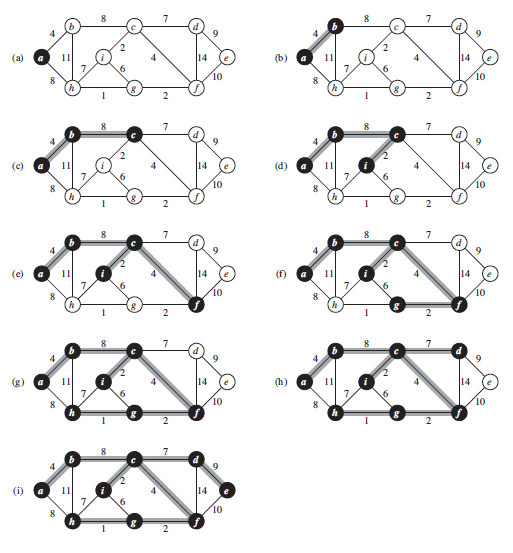
\includegraphics[width=\linewidth]{images/worksheet_4_solution_42.png}
            \end{center}
        \end{itemize}
    \end{itemize}

    \bigskip

    \underline{\textbf{References:}}

    \bigskip

    \begin{enumerate}[1)]
        \item Wikipedia, Kruskal Algorithm, \href{https://en.wikipedia.org/wiki/Kruskal%27s_algorithm}{link}
    \end{enumerate}

    \item

    \bigskip

    \begin{lstlisting}[mathescape=true]
    BELLMAN-FORD(G,w,s)
        INITIALIZE-SINGLE-SOURCE(G,s)
        active = true

        while(active)
            for each edge $(u,v) \in G.E$
                RELAX(u,v,w)

                if $v.d > u.d + w(u,v)$
                    return False

        return True


    RELAX(u,v,w)
        if v.d > u.d + w(u,v)
            v.d = u.d + w(u,v)
            $v.\pi$ = u
        else
            active = false
    \end{lstlisting}

    \bigskip

    \underline{\textbf{Notes:}}

    \bigskip

    \begin{itemize}
        \item $m$ here represents the total number of edges in shortest path
        between $u$ and $v$
        \item \textbf{Negative-Weight Cycle}

        \begin{itemize}
            \item Is a cycle with weights that sum to a negative number

            \begin{center}
            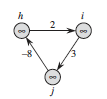
\includegraphics[width=0.35\linewidth]{images/worksheet_4_solution_43.png}
            \end{center}
        \end{itemize}


        \item \textbf{Bellman-Ford Algorithm}
        \begin{itemize}
            \item Solves the single-source shortest-paths problem in the general case
            in which edge weights may be negative.

            \begin{center}
            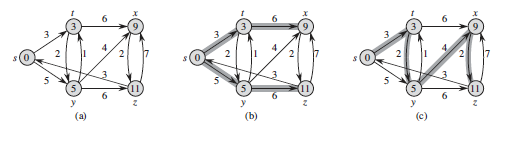
\includegraphics[width=\linewidth]{images/worksheet_4_solution_44.png}
            \end{center}

            \item Returns TRUE if and only if the graph contains no negative-weight cycles
            that are reachable from the source
        \end{itemize}
    \end{itemize}

    \item

    \begin{lstlisting}[mathescape=true]
    BELLMAN-FORD(G,w,s)
        INITIALIZE-SINGLE-SOURCE(G,s)
        for i = 1 to $\lvert G.V \rvert - 1$
            for each edge $(u,v) \in G.E$
                RELAX(u,v,w)

        for each edge $(u,v) \in G.E$
            if $v.d > u.d + w(u,v)$
                return False

        return True

    RELAX(u,v,w)
        if v.d > u.d + w(u,v)
            v.d = u.d + w(u,v)
            $v.\pi$ = u
        else
            v.d = -$\infty$
    \end{lstlisting}

    \item

    \bigskip

    I need to design algorithm that returns the most reliable path between two
    vertices.

    \bigskip

    \begin{lstlisting}[mathescape=true]
    DIJKSTRA(G,w,s)
        INITIALIZE-SINGLE-SOURCE(G,s)
        S = $\emptyset$
        Q = G.V

        while Q $\neq \emptyset$
            u = EXTRACT-MAX(Q)
            S = S $\cup$ {u}
            for each vertax v $\in$ G.Adj[u]
                RELAX(u,v,w)

    INITIALIZE-SINGLE-SOURCE(G,s)
        for each vertax v $\in$ G.V
            v.d = $-\infty$
            v.$\pi$ = NIL
        s.d = 1

    RELAX(u,v,w)
        if u.d * w(u,v) > v.d
            v.d = u.d * w(u,v)
            v.$\pi$ = u
    \end{lstlisting}

    \bigskip

    \underline{\textbf{Notes:}}

    \bigskip

    \begin{itemize}
        \item Dijkstra Algorithm
        \begin{itemize}
            \item Finds shortest path from one node to all nodes
            \item Solves the single-source shortest-paths problem on a weighted
            \underline{directed} graeph $G=(V,E)$
            \item Cannot have negative weight edges
        \end{itemize}

        \bigskip

        \begin{center}
        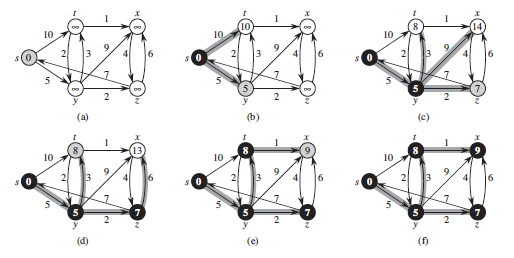
\includegraphics[width=0.7\linewidth]{images/worksheet_4_solution_45.png}
        \end{center}
    \end{itemize}

    \item

    \setcounter{equation}{0}

    \bigskip

    The output of the Floyd-Warshall algorithm can detect the presence
    of a negative weight cycle by looking for a negative value in the matrix $D^{(n)}$.

    \bigskip

    \underline{\textbf{Notes:}}

    \bigskip

    \begin{itemize}
        \item Floyd-Warshall Algorithm

        \begin{itemize}
            \item Is an algorithm for finding shortest paths between \underline{all} pairs of vertices in a weighted graph.
            \item Negative edges allowed
            \item Cannot have negative weight cycles
            \item Is useful in graphs with dense number of edges

            \begin{center}
            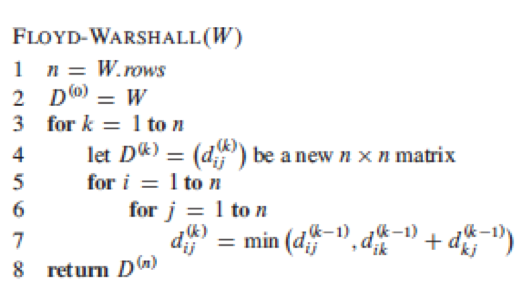
\includegraphics[width=0.5\linewidth]{images/worksheet_4_solution_46.png}
            \end{center}

            \begin{itemize}
                \item $n$: the number of vertices
                \item $W$: the $n \times n$ matrix of edge weights of an $n$-vertax directed graph $G = (V,E)$

                \begin{align}
                    w_{ij} &= \begin{cases}
                        0 & \text{if $i = j$}\\
                        \text{the weight of directed edge $(i,j)$)} & \text{if $i \neq j$ and $(i,j \in E)$}\\
                        \infty & \text{if $i \neq j$ and $(i,j) \notin E$}\\
                    \end{cases}
                \end{align}

                \item $D^{(k)}$: the $n \times n$ matrix of edge weights of shortest path
                where all intermediate vertices are in the set ${1,2,...,k}$.

                \begin{align}
                    d_{ij} &= \begin{cases}
                        w_{ij} & \text{if $k = 0$}\\
                        \text{min($d_{ij}^{(k-1)}, d_{ik}^{(k-1)} + d_{kj}^{(k-1)}$)} & \text{if $k \geq 1$}\\
                    \end{cases}
                \end{align}
            \end{itemize}

            \bigskip

            \underline{\textbf{Example:}}

            \bigskip

            \begin{center}
            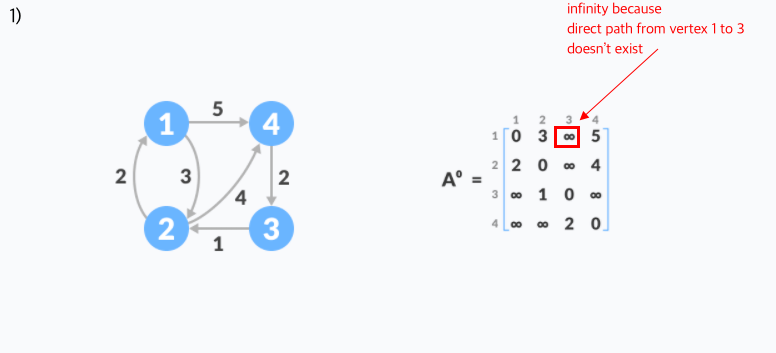
\includegraphics[width=\linewidth]{images/worksheet_4_solution_47.png}
            \end{center}

            \begin{itemize}
                \item $k = 1$

                \begin{center}
                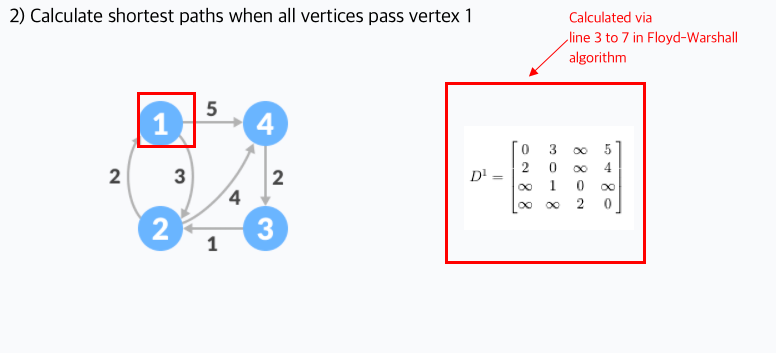
\includegraphics[width=0.5\linewidth]{images/worksheet_4_solution_48.png}
                \end{center}

                \begin{align}
                    D^1 = \begin{bmatrix}
                        0 & 3 & \infty & 5\\
                        2 & 0 & \infty & 4  \\
                        \infty & 1 & 0 & \infty \\
                        \infty & \infty & 2 & 0
                    \end{bmatrix}
                \end{align}

                \begin{itemize}
                    \item Matrix calculated via line 3 to 7 in Floyd-Warshall algorithm
                \end{itemize}

                \item $k = 2$

                \begin{center}
                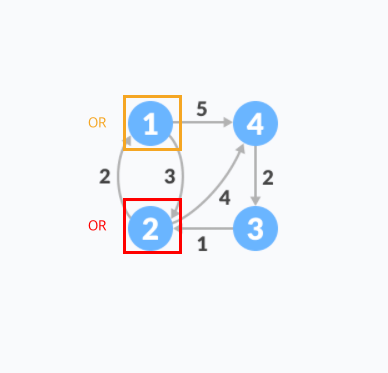
\includegraphics[width=0.5\linewidth]{images/worksheet_4_solution_49.png}
                \end{center}

                \begin{align}
                    D^2 = \begin{bmatrix}
                        0 & 3 & \infty & 5\\
                        2 & 0 & \infty & 4\\
                        \infty & 1 & 0 & 5\\
                        \infty & \infty & 2 & 0
                    \end{bmatrix}
                \end{align}

                \begin{itemize}
                    \item 5 in $D^2_{34}$ is the only value that's different
                \end{itemize}

                \item $k = 3$

                \begin{center}
                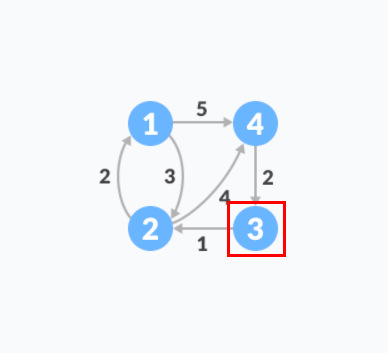
\includegraphics[width=0.5\linewidth]{images/worksheet_4_solution_50.png}
                \end{center}

                \begin{align}
                    D^3 = \begin{bmatrix}
                        0 & 2 & \infty & 4\\
                        2 & 0 & \infty & 4\\
                        \infty & 1 & 0 & 5\\
                        7 & 3 & 2 & 0
                    \end{bmatrix}
                \end{align}

                \item $k = 4$

                \begin{center}
                \includegraphics[width=0.5\linewidth]{images/worksheet_4_solution_51.png}
                \end{center}

                \begin{align}
                    D^4 = \begin{bmatrix}
                        0 & 3 & 7 & 5 \\
                        2 & 0 & 4 & 4 \\
                        12 & 1 & 0 & 5\\
                        7 & 3 & 2 & 0
                    \end{bmatrix}
                \end{align}
            \end{itemize}

            \bigskip

            \underline{\textbf{Example 2:}}

            \begin{center}
            \includegraphics[width=0.5\linewidth]{images/worksheet_4_solution_52.png}
            \end{center}

            \begin{align}
                W = \begin{bmatrix}
                    0 & -4\\
                    1 & 0
                \end{bmatrix}
            \end{align}

            \bigskip

            \begin{itemize}
                \item $k = 1$

                \begin{center}
                \includegraphics[width=0.5\linewidth]{images/worksheet_4_solution_53.png}
                \end{center}

                \begin{align}
                    W = \begin{bmatrix}
                        0 & -4\\
                        1 & 0
                    \end{bmatrix}
                \end{align}

                \item $k = 2$

                \begin{center}
                \includegraphics[width=0.5\linewidth]{images/worksheet_4_solution_54.png}
                \end{center}

                    \begin{align}
                        W = \begin{bmatrix}
                            0 & -4\\
                            1 & 0
                        \end{bmatrix}
                    \end{align}
            \end{itemize}
        \end{itemize}

    \end{itemize}

    \item
    \setcounter{equation}{0}
    \bigskip

    \underline{\textbf{Notes:}}

    \bigskip

    \begin{itemize}
        \item Johnson's Algorithm

        \begin{itemize}
            \item Is a way to find the shortest paths between all pairs of vertices
            in an edge-weighted, directed graph
            \item Allows some edges to be negative-number
            \item No negative-cycles may exist
            \item Is similar to Floyd-Warshall Algorithm
            \item Is most effective in graph with \underline{sparse} number of edges
            \item Works as a subroutine to Dijkstra and Bellman-Ford Algorithm
            \item Has running time of $O(nm + n(m + n log n)) = O(nm + nlog n)$
        \end{itemize}

        \item Reweighting
        \begin{itemize}
            \item Is a technique used in Johnson's Algorithm
            \item Is so that all edges have non-negative weights $^{[1]}$
        \end{itemize}

        \bigskip

        \underline{\textbf{Steps:}}

        \begin{enumerate}[1.]
            \item Create a source vertex $V' = V \cup \{s\}$ for some $s \notin V$ and $E' = E \cup \{(s,v): v \in V\}$
            \item Extend the weight functio $w$ so that $w(s,v) = 0$ for all $v \in V$

            \begin{center}
            \includegraphics[width=\linewidth]{images/worksheet_4_solution_55.png}
            \end{center}

            \item Reweight each edge $(u,v)$ with weight function $\hat{w}(u,v) = w(u,v) + h(u) - h(v)$

            \begin{center}
            \includegraphics[width=\linewidth]{images/worksheet_4_solution_56.png}
            \end{center}

            \bigskip

            \underline{Sample Calculations}

            \begin{align}
            \hat{w}(s, u_1) &= w(s, u_1) + h(s) - h(u_1)\\
            &= 0 + 0 - 0\\
            &= 0
            \end{align}

            \bigskip

            \begin{align}
            \hat{w}(s, u_2) &= w(s, u_2) + h(s) - h(u_2)\\
            &= 0 + 0 - (-1)\\
            &= 1
            \end{align}

            \bigskip

            \begin{align}
            \hat{w}(u_1, u_5) &= w(u_1, u_5) + h(u_1) - h(u_5)\\
            &= 0 + 0 - (-4)\\
            &= 4
            \end{align}

            \item Remove vertex $s$ and run Dijkstra's algorithm on every node in the graph

            \begin{center}
            \includegraphics[width=\linewidth]{images/worksheet_4_solution_57.png}
            \end{center}

            \begin{itemize}
                \item Apply Dijkstra's algorithm to calculate $\hat{\delta(u,v)}$

                \begin{center}
                \includegraphics[width=\linewidth]{images/worksheet_4_solution_60.png}
                \end{center}

                \bigskip

                \underline{NOTE!!}

                \bigskip

                \begin{itemize}
                    \item $\delta$ means shortest-path weights ($v.d$) derived from weight function $w$
                    \item $\hat{\delta}$ means shortest-path weights ($v.d$) derived from weight function $\hat{w}$

                    \begin{center}
                    \includegraphics[width=\linewidth]{images/worksheet_4_solution_59.png}
                    \end{center}
                \end{itemize}

                \item Convert each $\hat{\delta(u,v)}$ to $\delta(u,v)$
            \end{itemize}

            \bigskip
        \end{enumerate}
    \end{itemize}

    \bigskip

    \underline{\textbf{References}}

    \bigskip

    \begin{enumerate}[1)]
        \item Columbia University, Johnson’s Algorithm for All-Pairs Shortest Paths, \href{http://www.columbia.edu/~cs2035/courses/ieor6614.S16/johnson.pdf}{link}
    \end{enumerate}


\end{enumerate}

\end{document}